% vim: set spell spelllang=en tw=100 et sw=4 sts=4 foldmethod=marker foldmarker={{{,}}} :

\documentclass[aspectratio=169,compress,10pt]{beamer}

\usepackage{tikz}
\usepackage{xcolor}
\usepackage{complexity}
\usepackage{hyperref}
\usepackage{microtype}
\usepackage{amsmath}                   % \operatorname
\usepackage{amsfonts}                  % \mathcal
\usepackage{amssymb}                   % \nexists
\usepackage[vlined]{algorithm2e} % algorithms
\usepackage{centernot}
\usepackage{listings}
\usepackage{csquotes}
\usepackage{fancyvrb}
\usepackage{bussproofs}
\usepackage{multicol}
\usepackage{booktabs}
\usepackage{mathtools}
\usepackage{pifont}
\usepackage{marvosym}
\usepackage{cancel}

\usepackage{holtexbasic}
\usepackage{environ}
\NewEnviron{holthmenv}{%
  \scalebox{1.0}{\begin{array}[t]{l}
  \BODY
  \end{array}}}
\newcommand{\us}{\_}
\renewcommand{\HOLTokenTurnstile}{\ensuremath{\vdash\!\!}}
\renewcommand{\HOLConst}[1]{\textsf{\small #1}}
\renewcommand{\HOLFieldName}[1]{\textsf{\small #1}}
\renewcommand{\HOLSymConst}[1]{\HOLConst{#1}}
\renewcommand{\HOLTyOp}[1]{\HOLConst{#1}}
\renewcommand{\HOLinline}[1]{\textsf{\ensuremath{#1}}}
\renewcommand{\HOLKeyword}[1]{\ensuremath{\mathsf{#1}}}
\renewcommand{\HOLTokenBar}{\ensuremath{\mathtt{|}}}
\renewcommand{\HOLTokenLeftrec}{\ensuremath{\langle\!|}}
\renewcommand{\HOLTokenRightrec}{\ensuremath{|\!\rangle}}
\renewcommand{\HOLTokenLsl}{\raisebox{.15em}{\ensuremath{}\scriptsize{\textless\rule{-0.1em}{0em}\textless}{}}}

\renewcommand{\HOLStringLitDG}[1]{\scalebox{0.9}{\texttt{"#1"}}}
\renewcommand{\HOLStringLit}[1]{\scalebox{0.9}{\texttt{"#1"}}}
\renewcommand{\HOLCharLit}[1]{\scalebox{0.9}{\#\texttt{"#1"}}}
\newcommand{\HOLcount}[1]{\HOLTokenLeftbrace{}\HOLConst{0}\HOLSymConst{,}\HOLConst{1}\HOLSymConst{,}\HOLConst{...}\HOLSymConst{,}#1\HOLSymConst{\ensuremath{-}}\HOLConst{1}\HOLTokenRightbrace{}}

\usefonttheme{professionalfonts}

\usetikzlibrary{shapes, arrows, shadows, calc, positioning, fit}
\usetikzlibrary{decorations.pathreplacing, decorations.pathmorphing, shapes.misc}
\usetikzlibrary{tikzmark, backgrounds}
\usetikzlibrary{trees, overlay-beamer-styles}
\usetikzlibrary{backgrounds, scopes, graphs, graphs.standard, shapes.geometric}
\usetikzlibrary{shapes.multipart, arrows, arrows.meta, decorations, decorations.markings}

\tikzset{processarrow/.style={->, very thick, decorate, decoration={snake, post length=0.5mm}}}
\tikzset{brace/.style={decorate, decoration={brace}, very thick}}

\definecolor{uofguniversityblue}{rgb}{0, 0.219608, 0.396078}
\definecolor{uofgheather}{rgb}{0.356863, 0.32549, 0.490196}
\definecolor{uofgaquamarine}{rgb}{0.603922, 0.72549, 0.678431}
\definecolor{uofgslate}{rgb}{0.309804, 0.34902, 0.380392}
\definecolor{uofgrose}{rgb}{0.823529, 0.470588, 0.709804}
\definecolor{uofgmocha}{rgb}{0.709804, 0.564706, 0.47451}
\definecolor{uofgsandstone}{rgb}{0.321569, 0.278431, 0.231373}
\definecolor{uofgforest}{rgb}{0, 0.2, 0.129412}
\definecolor{uofglawn}{rgb}{0.517647, 0.741176, 0}
\definecolor{uofgcobalt}{rgb}{0, 0.615686, 0.92549}
\definecolor{uofgturquoise}{rgb}{0, 0.709804, 0.819608}
\definecolor{uofgsunshine}{rgb}{1.0, 0.862745, 0.211765}
\definecolor{uofgpumpkin}{rgb}{1.0, 0.72549, 0.282353}
\definecolor{uofgthistle}{rgb}{0.584314, 0.070588, 0.447059}
\definecolor{uofgrust}{rgb}{0.603922, 0.227451, 0.023529}
\definecolor{uofgburgundy}{rgb}{0.490196, 0.133333, 0.223529}
\definecolor{uofgpillarbox}{rgb}{0.701961, 0.047059, 0}
\definecolor{uofglavendar}{rgb}{0.356863, 0.301961, 0.580392}
\definecolor{uofgleaf}{rgb}{0, 0.517647, 0.239216}

% {{{ theme things
\useoutertheme[footline=authortitle]{miniframes}
\useinnertheme{rectangles}

\setbeamerfont{block title}{size={}}
\setbeamerfont{title}{size=\large,series=\bfseries}
\setbeamerfont{section title}{size=\large,series=\mdseries}
\setbeamerfont{author}{size=\normalsize,series=\mdseries}
\setbeamercolor*{structure}{fg=uofguniversityblue}
\setbeamercolor*{palette primary}{use=structure,fg=black,bg=white}
\setbeamercolor*{palette secondary}{use=structure,fg=white,bg=uofgcobalt}
\setbeamercolor*{palette tertiary}{use=structure,fg=white,bg=uofguniversityblue}
\setbeamercolor*{palette quaternary}{fg=white,bg=black}
\setbeamercolor{block body}{bg=structure!10}
\setbeamercolor{block title}{bg=structure,fg=white}
\setbeamertemplate{blocks}[rounded]
\setbeamercolor*{titlelike}{parent=palette primary}

\beamertemplatenavigationsymbolsempty
\setbeamersize{text margin left=0.5cm}
\setbeamersize{text margin right=0.5cm}

\setbeamertemplate{title page}
{
    \begin{tikzpicture}[remember picture, overlay]
        \node at (current page.north west) {
            \begin{tikzpicture}[remember picture, overlay]
                \fill [fill=uofguniversityblue, anchor=north west] (0, 0) rectangle (\paperwidth, -2.6cm);
            \end{tikzpicture}
        };

        \node (logo) [anchor=north east, shift={(-0.8cm,-0.2cm)}] at (current page.north east) {
            
\includegraphics[keepaspectratio=true,scale=0.5]{../../images/UoG_keyline.pdf}
        };

        \node (logo2) [anchor=north, below=0.2cm of logo.south] {
            
\includegraphics[keepaspectratio=true,scale=0.1]{../../images/RAEngWhite.pdf}
        };

        \coordinate (logos) at ($(logo.south)!0.5!(logo2.north)$);

        \node [anchor=west, xshift=0.8cm] at (current page.west |- logos) {
            \begin{minipage}{0.65\paperwidth}\raggedright
                {\usebeamerfont{title}\usebeamercolor[white]{}\inserttitle}\\[0.2cm]
                {\usebeamerfont{author}\usebeamercolor[white]{}\insertauthor}
            \end{minipage}
        };
    \end{tikzpicture}
}

\setbeamertemplate{section page}
{
    \begin{centering}
        \begin{beamercolorbox}[sep=12pt,center]{part title}
            \usebeamerfont{section title}\insertsection\par
        \end{beamercolorbox}
    \end{centering}
}

\newcommand{\frameofframes}{/}
\newcommand{\setframeofframes}[1]{\renewcommand{\frameofframes}{#1}}

\makeatletter
\setbeamertemplate{footline}
{%
    \begin{beamercolorbox}[colsep=1.5pt]{upper separation line foot}
    \end{beamercolorbox}
    \begin{beamercolorbox}[ht=2.5ex,dp=1.125ex,%
        leftskip=.3cm,rightskip=.3cm plus1fil]{title in head/foot}%
        {\usebeamerfont{title in head/foot}\insertshorttitle}%
        \hspace{0.22\textwidth}%
        {\usebeamerfont{author in head/foot}\insertshortauthor}%
        \hfill%
        {\usebeamerfont{frame number}\usebeamercolor[fg]{frame number}\insertframenumber~\frameofframes~\inserttotalframenumber}
    \end{beamercolorbox}%
    \begin{beamercolorbox}[colsep=1.5pt]{lower separation line foot}
    \end{beamercolorbox}
}

\makeatletter
\setbeamertemplate{mini frame}
{%
  \begin{pgfpicture}{0pt}{0pt}{.04cm}{.04cm}
    \pgfpathcircle{\pgfpoint{0.04cm}{0.04cm}}{0.04cm}
    \pgfusepath{fill,stroke}
  \end{pgfpicture}%
}
\setbeamertemplate{mini frame in current subsection}
{%
  \begin{pgfpicture}{0pt}{0pt}{.04cm}{.04cm}
    \pgfpathcircle{\pgfpoint{0.04cm}{0.04cm}}{0.04cm}
    \pgfsetfillcolor{section in head/foot.bg}
    \pgfusepath{fill,stroke}
  \end{pgfpicture}%
}

\setbeamersize{mini frame size=0.10cm, mini frame offset=0.06cm}
\makeatother

\makeatletter
\newenvironment{nearlyplainframe}[2][]{
    \def\beamer@entrycode{\vspace*{-\headheight}\vspace*{3pt}}
    \setbeamertemplate{headline}
    {%
        \begin{beamercolorbox}[colsep=1.5pt]{upper separation line head}
        \end{beamercolorbox}
        \begin{beamercolorbox}[ht=0.5ex,dp=0.125ex,%
            leftskip=.3cm,rightskip=.3cm plus1fil]{title in head/foot}%
        \end{beamercolorbox}%
        \begin{beamercolorbox}[ht=0.5ex,dp=0.125ex,%
            leftskip=.3cm,rightskip=.3cm plus1fil]{author in head/foot}%
        \end{beamercolorbox}%
        \begin{beamercolorbox}[colsep=1.5pt]{lower separation line head}
        \end{beamercolorbox}
        \vspace*{\headheight}
    }

    \setbeamertemplate{footline}
    {%
        \begin{beamercolorbox}[colsep=1.5pt]{upper separation line foot}
        \end{beamercolorbox}
        \begin{beamercolorbox}[ht=0.5ex,dp=0.125ex,%
            leftskip=.3cm,rightskip=.3cm plus1fil]{author in head/foot}%
        \end{beamercolorbox}%
        \begin{beamercolorbox}[ht=0.5ex,dp=0.125ex,%
            leftskip=.3cm,rightskip=.3cm plus1fil]{title in head/foot}%
        \end{beamercolorbox}%
        \begin{beamercolorbox}[colsep=1.5pt]{lower separation line foot}
        \end{beamercolorbox}
    }

    \begin{frame}[#1]{#2}
    }{
    \end{frame}
}
\makeatother

% }}}

\tikzstyle{state} = [inner sep=1pt]
\tikzstyle{infeasible} = [color=uofgpillarbox]
\tikzstyle{dominated} = [color=uofgcobalt]
\tikzstyle{backwards} = []
\tikzstyle{accept} = [solid, thick]
\tikzstyle{reject} = [dotted, thick]
\tikzstyle{forced} = [color=uofglawn]
\tikzstyle{domination} = [dashed, thick, ->, color=uofgcobalt]

\newcommand{\set}[1]{\{ #1 \}}
\newcommand{\setsize}[1]{{\left|#1\right|}}

\newcommand{\solvernameformat}[1]{\textit{#1}}
\newcommand{\toolformat}[1]{\textit{#1}}
\newcommand{\proofsystemformat}[1]{\textsc{#1}\@}

\newcommand{\veripb}{\toolformat{VeriPB}\xspace}
\renewcommand{\veripb}{\proofsystemformat{VeriPB}\xspace}
\newcommand\veripbid[1]{\alertred{#1}}
\newcommand\veripbConstraint[1]{\alertblue{#1}}

\newcommand{\neighbourhood}{\operatorname{N}}
\newcommand{\vertexset}{\operatorname{V}}
\newcommand{\degree}{\operatorname{deg}}

\providecommand{\reifvar}{r}
\providecommand{\reifimpllft}{\Leftarrow}
\providecommand{\reifimplrt}{\Rightarrow}
\providecommand{\reifequiv}{\Leftrightarrow}
\providecommand{\reifconstrlft}[2]{#1 \reifimpllft #2}
\providecommand{\reifconstrrt}[2]{#1 \reifimplrt #2}
\providecommand{\reifconstrequiv}[2]{#1 \reifequiv #2}

\newcommand{\colorblue}[1]{\textcolor{uofgcobalt}{#1}}
\newcommand{\colorred}[1]{\textcolor{uofgthistle}{#1}}
\newcommand{\colorgreen}[1]{\textcolor{uofglawn}{#1}}

% For highlighting in examples
%   \newcommand<>{\alertred}[1]{{\color#2{red}#1}}
\newcommand<>{\alertred}[1]{{\color#2{uofgthistle}#1}}
\renewcommand<>{\alert}[1]{{\color#2{uofgthistle}#1}}
%   \newcommand<>{\alertblue}[1]{{\color#2[rgb]{0,0,0.7}#1}}
\newcommand<>{\alertblue}[1]{{\color#2{uofgcobalt}#1}}
%   \newcommand<>{\alertgreen}[1]{{\color#2[rgb]{0,0.6,0}#1}}
\newcommand<>{\alertgreen}[1]{{\color#2{uofglawn}#1}}

%%% Extra alert command colours
\newcommand<>{\alertlav}[1]{{\color#2{uofglavendar}#1}}
% Pillarbox is kind of red
\newcommand<>{\alertpillarbox}[1]{{\color#2{uofgpillarbox}#1}}
% Pumpkin is kind of orange
\newcommand<>{\alertpumpkin}[1]{{\color#2{uofgpumpkin}#1}}
\newcommand<>{\alertorange}[1]{{\color#2{uofgpumpkin}#1}}

%%% White text to reserve right amount of space
\newcommand<>{\alertwhite}[1]{{\color#2{white}#1}}

\author{Ciaran McCreesh}
\title{Proof Logging for Subgraph-Finding Algorithms}

\begin{document}

{
    \usebackgroundtemplate{
        \tikz[overlay, remember picture]
        \node[at=(current page.south), anchor=south, inner sep=0pt, yshift=-1.4cm]{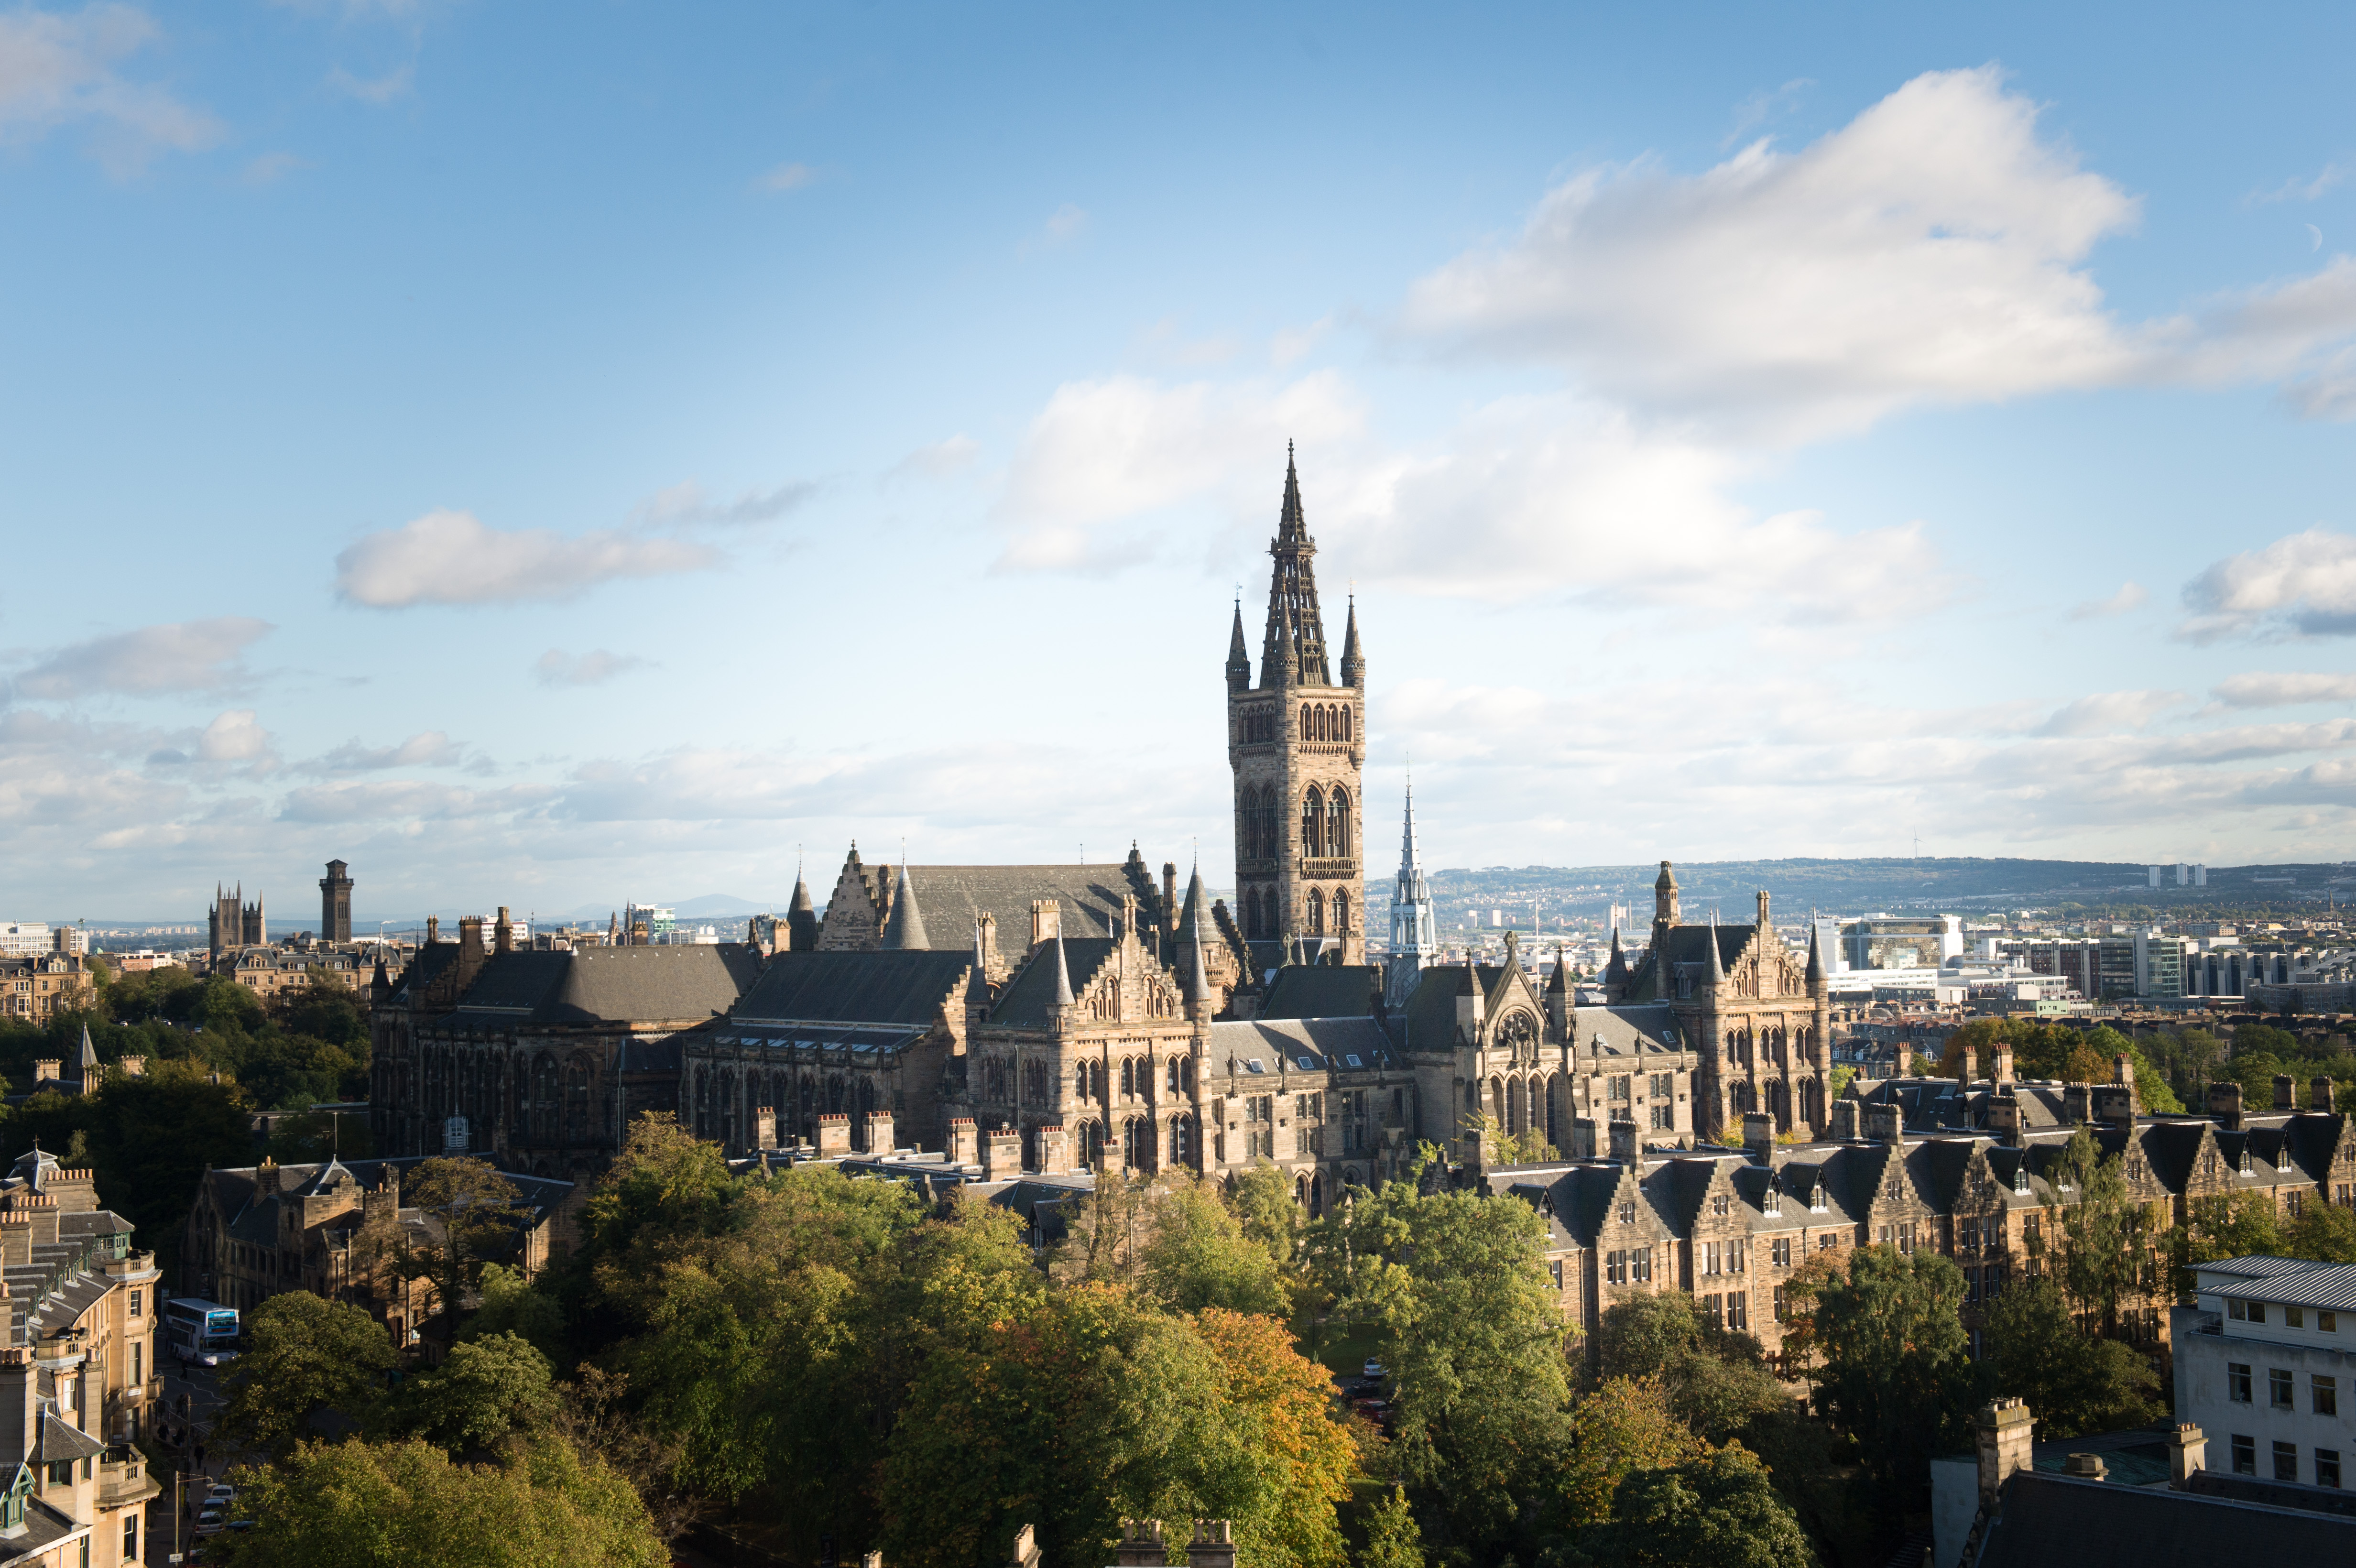
\includegraphics[keepaspectratio=true, width=\paperwidth]{../../images/background.jpg}};
    }
    \begin{frame}[plain,noframenumbering]
        \titlepage
    \end{frame}
}

\section{Maximum Clique}

\begin{frame}{Maximum Clique}
    \centering
    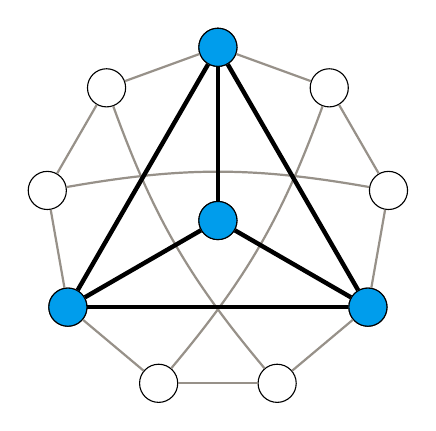
\begin{tikzpicture}
        \newcount \myc
        \foreach \n in {1, ..., 9}{
            \myc=\n \advance\myc by -1 \multiply\myc by -360 \divide\myc by 9 \advance\myc by 290
            \ifthenelse{\n = 3 \OR \n = 6 \OR \n = 9}{
                \node<1>[draw, circle, inner sep=2pt] (N\n) at (\the\myc:2.2) {\phantom{0}};
                \node<2>[draw, circle, fill=uofgcobalt, inner sep=2pt] (N\n) at (\the\myc:2.2) {\phantom{0}};
            }{
                \node[draw, circle, fill=white, inner sep=2pt] (N\n) at (\the\myc:2.2) {\phantom{0}};
            }
        }
        \node<1>[draw, circle, inner sep=2pt] (N10) at (0, 0) {\phantom{0}};
        \node<2>[draw, circle, fill=uofgcobalt, inner sep=2pt] (N10) at (0, 0) {\phantom{0}};

        \draw [thick, color=uofgsandstone!60] (N1) -- (N2);
        \draw [thick, color=uofgsandstone!60] (N2) -- (N3);
        \draw [thick, color=uofgsandstone!60] (N3) -- (N4);
        \draw [thick, color=uofgsandstone!60] (N4) -- (N5);
        \draw [thick, color=uofgsandstone!60] (N5) -- (N6);
        \draw [thick, color=uofgsandstone!60] (N6) -- (N7);
        \draw [thick, color=uofgsandstone!60] (N7) -- (N8);
        \draw [thick, color=uofgsandstone!60] (N8) -- (N9);
        \draw [thick, color=uofgsandstone!60] (N9) -- (N1);

        \draw [thick, color=uofgsandstone!60] (N4) to [out=10, in=170] (N8);
        \draw [thick, color=uofgsandstone!60] (N2) to [out=50, in=250] (N7);
        \draw [thick, color=uofgsandstone!60] (N5) to [out=290, in=130] (N1);

        \draw<1> [thick, color=uofgsandstone!60] (N3) -- (N10);
        \draw<2> [ultra thick] (N3) -- (N10);
        \draw<1> [thick, color=uofgsandstone!60] (N6) -- (N10);
        \draw<2> [ultra thick] (N6) -- (N10);
        \draw<1> [thick, color=uofgsandstone!60] (N9) -- (N10);
        \draw<2> [ultra thick] (N9) -- (N10);
        \draw<1> [thick, color=uofgsandstone!60] (N6) -- (N3);
        \draw<2> [ultra thick] (N6) -- (N3);
        \draw<1> [thick, color=uofgsandstone!60] (N9) -- (N3);
        \draw<2> [ultra thick] (N9) -- (N3);
        \draw<1> [thick, color=uofgsandstone!60] (N6) -- (N9);
        \draw<2> [ultra thick] (N6) -- (N9);
    \end{tikzpicture}
\end{frame}

\begin{frame}{A Brief and Incomplete Guide to Clique Solving (1/4)}
  Recursive maximum clique algorithm:
  \begin{itemize}
  \item Pick a vertex $v$.
  \item Either $v$ is in the clique\ldots
    \begin{itemize}
    \item Throw away every vertex not adjacent to $v$.
    \item If vertices remain, recurse.
    \end{itemize}
  \item \ldots{}or $v$ is not in the clique, so
    \begin{itemize}
    \item Throw $v$ away and pick another vertex.
    \end{itemize}
  \end{itemize}
\end{frame}

\begin{frame}{A Brief and Incomplete Guide to Clique Solving (2/4)}
  Key data structures:
  \begin{itemize}
  \item Growing clique $C$.
  \item Shrinking set of potential vertices $P$.
    \begin{itemize}
    \item All the vertices we haven't thrown away yet.
    \item Every $v \in P$ is adjacent to every $w \in C$.
    \end{itemize}
  \end{itemize}
  \bigskip
  \uncover<2->{
    Branch and bound:
    \begin{itemize}
    \item Remember the biggest clique
%                     found so far, $C^\star$.
      $C^\star$ found so far.
    \item
      If
      $
      \setsize{C} + \setsize{P} \le \setsize{C^\star}
      $,
      no need to keep going.
    \end{itemize}
  }
\end{frame}

\begin{frame}{A Brief and Incomplete Guide to Clique Solving (3/4)}
  \begin{center}
    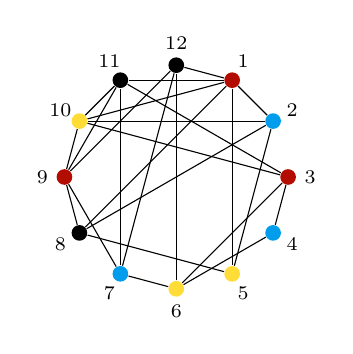
\begin{tikzpicture}
      \begin{scope}[every node/.style = {font=\scriptsize}]
        \newcount \myc
        \foreach \n in {1, 3, 9}{
          \myc=\n \advance\myc by -1 \multiply\myc by -360 \divide\myc by 12 \advance\myc by 60
          \node[anchor=center] (L\n) at (\the\myc:1.7) {\n};
          \node[anchor=center, circle, fill=uofgpillarbox, inner sep=2pt] (N\n) at (\the\myc:1.42) {};
        }
        \foreach \n in {2, 4, 7}{
          \myc=\n \advance\myc by -1 \multiply\myc by -360 \divide\myc by 12 \advance\myc by 60
          \node[anchor=center] (L\n) at (\the\myc:1.7) {\n};
          \node[anchor=center, circle, fill=uofgcobalt, inner sep=2pt] (N\n) at (\the\myc:1.42) {};
        }
        \foreach \n in {5, 6, 10}{
          \myc=\n \advance\myc by -1 \multiply\myc by -360 \divide\myc by 12 \advance\myc by 60
          \node[anchor=center] (L\n) at (\the\myc:1.7) {\n};
          \node[anchor=center, circle, fill=uofgsunshine, inner sep=2pt] (N\n) at (\the\myc:1.42) {};
        }
        \foreach \n in {8, 11, 12}{
          \myc=\n \advance\myc by -1 \multiply\myc by -360 \divide\myc by 12 \advance\myc by 60
          \node[anchor=center] (L\n) at (\the\myc:1.7) {\n};
          \node[anchor=center, circle, fill=black, inner sep=2pt] (N\n) at (\the\myc:1.42) {};
        }
        \draw (N1) -- (N2);
        \draw (N1) -- (N5);
        \draw (N1) -- (N8);
        \draw (N1) -- (N10);
        \draw (N1) -- (N11);
        \draw (N1) -- (N12);
        \draw (N2) -- (N5);
        \draw (N2) -- (N8);
        \draw (N2) -- (N10);
        \draw (N3) -- (N4);
        \draw (N3) -- (N6);
        \draw (N3) -- (N10);
        \draw (N3) -- (N11);
        \draw (N4) -- (N6);
        \draw (N5) -- (N8);
        \draw (N6) -- (N7);
        \draw (N6) -- (N12);
        \draw (N7) -- (N9);
        \draw (N7) -- (N11);
        \draw (N7) -- (N12);
        \draw (N8) -- (N9);
        \draw (N9) -- (N10);
        \draw (N9) -- (N11);
        \draw (N9) -- (N12);
        \draw (N10) -- (N11);
      \end{scope}
    \end{tikzpicture}
  \end{center}

  Given a $k$-colouring of a subgraph, that subgraph cannot have a clique of more than
  $k$ vertices.

  \medskip

  We can use $\setsize{C} + \mathit{\#colours}(P)$ as a bound, for any colouring.

\end{frame}

\begin{frame}{A Brief and Incomplete Guide to Clique Solving (4/4)}
  \begin{itemize}
  \item
    This brings us to 1997.
    \medskip
  \item
%       In practice, better bound functions, clever vertex selection
%       heuristics, efficient data structures, local search, \ldots
    Many improvements since then:
    \begin{itemize}
    \item
      better bound functions,
    \item
      clever vertex selection heuristics,
    \item
    efficient data structures,
    \item
    local search,
    \item
      \ldots
    \end{itemize}
    \medskip
  \item
    But key ideas for proof logging can be explained without worrying about such things.
  \end{itemize}
\end{frame}

\begin{frame}{Why I'm Here\ldots}
\end{frame}

\section{Proof Logging}

\begin{frame}{Proof Logging}
    \vspace*{-1.0em}
    \begin{center}
        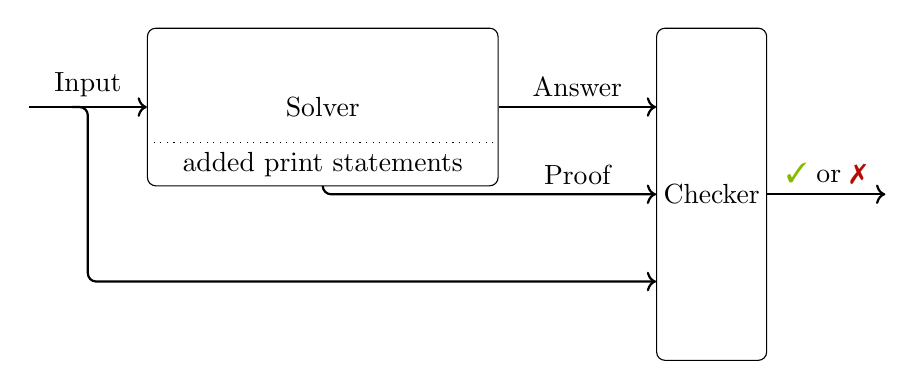
\begin{tikzpicture}
            \node (solver) [inner xsep=5em, inner ysep=2.5em, draw, rounded corners=3pt] { Solver };

            \node (checker) [right=2cm of solver.north east, anchor=north west, inner xsep=0.25em, draw, rounded corners=3pt, minimum height=12em, visible on=<3->] { Checker };

            \node (print) [anchor=south, above=0cm of solver.south, visible on=<2->] { added print statements };
            \draw [dotted, visible on=<2->] (solver.west|-print.north) -- (solver.east|-print.north);

            \draw [->, thick] (solver.east) -- (solver.east -| checker.west)
                coordinate [midway] (solutionmid) node [above, midway] { Answer };

            \draw [->, thick, rounded corners=3pt, visible on=<2->] (solver.south) -- (solver.south |- checker.west)
                -- (checker.west) coordinate [midway] (proofmid);

            \coordinate (prooflabel) at (proofmid-|solutionmid);
            \node [above=0cm of prooflabel, visible on=<2->] { Proof };

            \coordinate [right=1.5cm of checker.east] (verified);
            \draw [->, thick, visible on=<4->] (checker.east) -- (verified) node [above, midway] { \textcolor{uofglawn}{\ding{51}} or \textcolor{uofgpillarbox}{\ding{55}} };

            \coordinate [left=1.5cm of solver.west] (input);
            \draw [->, thick] (input) -- (solver.west) coordinate [midway] (inputmid) node [above, midway] { Input };

            \coordinate (checkerbotleft) at ($(checker.west)+($(checker.west)-(solver.east-|checker.west)$)$);

            \draw [->, thick, rounded corners=3pt, visible on=<3->] ($(inputmid)+(-0.2,0)$) -- (inputmid) -- (inputmid |- checkerbotleft) -- (checkerbotleft);
        \end{tikzpicture}
      \end{center}
    \vspace*{-0.7em}
  \begin{enumerate}
  \item<1->
    Run solver on problem input.
  \item<2->
    Solver also prints out a proof as part of its output.
  \item<3->
    Feed input + solution + proof to proof checker.
  \item<4->
    Verify that proof checker says solution is correct.
  \end{enumerate}
\end{frame}

\begin{frame}{What is a Proof?}
\end{frame}

\begin{frame}[fragile,t]{What Might an Ad-Hoc Proof Look Like?}%
\only<2>{
\begin{tikzpicture}[overlay,remember picture] \coordinate (ahcliqueheader1space) at ($(pic cs:ahcliqueheader1)+(0pt,4pt)$); \node[rounded corners, fit = (ahcliqueheader1space) (pic cs:ahcliqueheader2), fill=uofgsunshine] {};\end{tikzpicture}}%
\only<6>{
\begin{tikzpicture}[overlay,remember picture] \coordinate (ahopt1space) at ($(pic cs:ahopt1a)+(0pt,4pt)$); \node[rounded corners, fit = (ahopt1space) (pic cs:ahopt1b), fill=uofgsunshine] {};\end{tikzpicture}}%
\only<7>{
\begin{tikzpicture}[overlay,remember picture] \coordinate (ahbt1space) at ($(pic cs:ahbt1a)+(0pt,4pt)$); \node[rounded corners, fit = (ahbt1space) (pic cs:ahbt1b), fill=uofgsunshine] {};\end{tikzpicture}}%
\only<8>{
\begin{tikzpicture}[overlay,remember picture] \coordinate (ahbt2space) at ($(pic cs:ahbt2a)+(0pt,4pt)$); \node[rounded corners, fit = (ahbt2space) (pic cs:ahbt2b), fill=uofgsunshine] {};\end{tikzpicture}}%
\only<9>{
\begin{tikzpicture}[overlay,remember picture] \coordinate (ahbt3space) at ($(pic cs:ahbt3a)+(0pt,4pt)$); \node[rounded corners, fit = (ahbt3space) (pic cs:ahbt3b), fill=uofgsunshine] {};\end{tikzpicture}}%
\only<10>{
\begin{tikzpicture}[overlay,remember picture] \coordinate (ahbt4space) at ($(pic cs:ahbt4a)+(0pt,4pt)$); \node[rounded corners, fit = (ahbt4space) (pic cs:ahbt4b), fill=uofgsunshine] {};\end{tikzpicture}}%
\only<11>{
\begin{tikzpicture}[overlay,remember picture] \coordinate (ahopt2space) at ($(pic cs:ahopt2a)+(0pt,4pt)$); \node[rounded corners, fit = (ahopt2space) (pic cs:ahopt2b), fill=uofgsunshine] {};\end{tikzpicture}}%
\only<12>{
\begin{tikzpicture}[overlay,remember picture] \coordinate (ahbt5space) at ($(pic cs:ahbt5a)+(0pt,4pt)$); \node[rounded corners, fit = (ahbt5space) (pic cs:ahbt5b), fill=uofgsunshine] {};\end{tikzpicture}}%
\only<13>{
\begin{tikzpicture}[overlay,remember picture] \coordinate (ahbt6space) at ($(pic cs:ahbt6a)+(0pt,4pt)$); \node[rounded corners, fit = (ahbt6space) (pic cs:ahbt6b), fill=uofgsunshine] {};\end{tikzpicture}}%
\only<14>{
\begin{tikzpicture}[overlay,remember picture] \coordinate (ahbt7space) at ($(pic cs:ahbt7a)+(0pt,4pt)$); \node[rounded corners, fit = (ahbt7space) (pic cs:ahbt7b), fill=uofgsunshine] {};\end{tikzpicture}}%
\only<15>{
\begin{tikzpicture}[overlay,remember picture] \coordinate (ahcontaspace) at ($(pic cs:ahconta)+(0pt,4pt)$); \node[rounded corners, fit = (ahcontaspace) (pic cs:ahcontb), fill=uofgsunshine] {};\end{tikzpicture}}%
\begin{tikzpicture}[overlay,remember picture]
    \node [xshift=-3cm, yshift=0.5cm] at (current page.east) {
        \begin{tikzpicture}
    \begin{scope}[every node/.style = {font=\scriptsize}]

        \myc=1 \advance\myc by -1 \multiply\myc by -360 \divide\myc by 12 \advance\myc by 60
        \node[anchor=center] (L1) at (\the\myc:1.7) {1};
        \node<1-3>[anchor=center, circle, fill=black, inner sep=2pt] (N1) at (\the\myc:1.42) {};
        \node<4-6>[anchor=center, circle, fill=black!20, inner sep=2pt] (N1) at (\the\myc:1.42) {};
        \node<7>[anchor=center, circle, fill=black!20, inner sep=2pt] (N1) at (\the\myc:1.42) {};
        \node<8>[anchor=center, circle, fill=black, inner sep=2pt] (N1) at (\the\myc:1.42) {};
        \node<9-10>[anchor=center, circle, fill=black, inner sep=2pt] (N1) at (\the\myc:1.42) {};
        \node<11>[anchor=center, circle, fill=uofgcobalt, inner sep=2pt] (N1) at (\the\myc:1.42) {};
        \node<12->[anchor=center, circle, fill=black, inner sep=2pt] (N1) at (\the\myc:1.42) {};

        \myc=2 \advance\myc by -1 \multiply\myc by -360 \divide\myc by 12 \advance\myc by 60
        \node[anchor=center] (L2) at (\the\myc:1.7) {2};
        \node<1-2>[anchor=center, circle, fill=black, inner sep=2pt] (N2) at (\the\myc:1.42) {};
        \node<3-10>[anchor=center, circle, fill=black!20, inner sep=2pt] (N2) at (\the\myc:1.42) {};
        \node<11>[anchor=center, circle, fill=uofgcobalt, inner sep=2pt] (N2) at (\the\myc:1.42) {};
        \node<12->[anchor=center, circle, fill=black, inner sep=2pt] (N2) at (\the\myc:1.42) {};

        \myc=3 \advance\myc by -1 \multiply\myc by -360 \divide\myc by 12 \advance\myc by 60
        \node[anchor=center] (L3) at (\the\myc:1.7) {3};
        \node<1-2>[anchor=center, circle, fill=black, inner sep=2pt] (N3) at (\the\myc:1.42) {};
        \node<3-6>[anchor=center, circle, fill=black!20, inner sep=2pt] (N3) at (\the\myc:1.42) {};
        \node<7>[anchor=center, circle, fill=black!20, inner sep=2pt] (N3) at (\the\myc:1.42) {};
        \node<8>[anchor=center, circle, fill=black!20, inner sep=2pt] (N3) at (\the\myc:1.42) {};
        \node<9-10>[anchor=center, circle, fill=black, inner sep=2pt] (N3) at (\the\myc:1.42) {};
        \node<11-13>[anchor=center, circle, fill=black!20, inner sep=2pt] (N3) at (\the\myc:1.42) {};
        \node<14->[anchor=center, circle, fill=black, inner sep=2pt] (N3) at (\the\myc:1.42) {};

        \myc=4 \advance\myc by -1 \multiply\myc by -360 \divide\myc by 12 \advance\myc by 60
        \node[anchor=center] (L4) at (\the\myc:1.7) {4};
        \node<1-2>[anchor=center, circle, fill=black, inner sep=2pt] (N4) at (\the\myc:1.42) {};
        \node<3-13>[anchor=center, circle, fill=black!20, inner sep=2pt] (N4) at (\the\myc:1.42) {};
        \node<14->[anchor=center, circle, fill=black, inner sep=2pt] (N4) at (\the\myc:1.42) {};

        \myc=5 \advance\myc by -1 \multiply\myc by -360 \divide\myc by 12 \advance\myc by 60
        \node[anchor=center] (L5) at (\the\myc:1.7) {5};
        \node<1-2>[anchor=center, circle, fill=black, inner sep=2pt] (N5) at (\the\myc:1.42) {};
        \node<3-10>[anchor=center, circle, fill=black!20, inner sep=2pt] (N5) at (\the\myc:1.42) {};
        \node<11>[anchor=center, circle, fill=uofgcobalt, inner sep=2pt] (N5) at (\the\myc:1.42) {};
        \node<12>[anchor=center, circle, fill=uofgthistle, inner sep=2pt] (N5) at (\the\myc:1.42) {};
        \node<13>[anchor=center, circle, fill=black!20, inner sep=2pt] (N5) at (\the\myc:1.42) {};
        \node<14->[anchor=center, circle, fill=black, inner sep=2pt] (N5) at (\the\myc:1.42) {};

        \myc=6 \advance\myc by -1 \multiply\myc by -360 \divide\myc by 12 \advance\myc by 60
        \node[anchor=center] (L6) at (\the\myc:1.7) {6};
        \node<1-4>[anchor=center, circle, fill=black, inner sep=2pt] (N6) at (\the\myc:1.42) {};
        \node<5-6>[anchor=center, circle, fill=black!20, inner sep=2pt] (N6) at (\the\myc:1.42) {};
        \node<7-8>[anchor=center, circle, fill=black, inner sep=2pt] (N6) at (\the\myc:1.42) {};
        \node<9-13>[anchor=center, circle, fill=black!20, inner sep=2pt] (N6) at (\the\myc:1.42) {};
        \node<14->[anchor=center, circle, fill=black, inner sep=2pt] (N6) at (\the\myc:1.42) {};

        \myc=7 \advance\myc by -1 \multiply\myc by -360 \divide\myc by 12 \advance\myc by 60
        \node[anchor=center] (L7) at (\the\myc:1.7) {7};
        \node<1-3>[anchor=center, circle, fill=black, inner sep=2pt] (N7) at (\the\myc:1.42) {};
        \node<4-6>[anchor=center, circle, fill=uofgcobalt, inner sep=2pt] (N7) at (\the\myc:1.42) {};
        \node<7>[anchor=center, circle, fill=uofgthistle, inner sep=2pt] (N7) at (\the\myc:1.42) {};
        \node<8-9>[anchor=center, circle, fill=black!20, inner sep=2pt] (N7) at (\the\myc:1.42) {};
        \node<10>[anchor=center, circle, fill=black, inner sep=2pt] (N7) at (\the\myc:1.42) {};
        \node<11-13>[anchor=center, circle, fill=black!20, inner sep=2pt] (N7) at (\the\myc:1.42) {};
        \node<14->[anchor=center, circle, fill=black, inner sep=2pt] (N7) at (\the\myc:1.42) {};

        \myc=8 \advance\myc by -1 \multiply\myc by -360 \divide\myc by 12 \advance\myc by 60
        \node<1-13>[anchor=center] (L8) at (\the\myc:1.7) {8};
        \node<14->[anchor=center] (L8) at (\the\myc:1.7) {\phantom{8}};
        \node<1-2>[anchor=center, circle, fill=black, inner sep=2pt] (N8) at (\the\myc:1.42) {};
        \node<3-10>[anchor=center, circle, fill=black!20, inner sep=2pt] (N8) at (\the\myc:1.42) {};
        \node<11>[anchor=center, circle, fill=uofgcobalt, inner sep=2pt] (N8) at (\the\myc:1.42) {};
        \node<12-13>[anchor=center, circle, fill=uofgthistle, inner sep=2pt] (N8) at (\the\myc:1.42) {};

        \myc=9 \advance\myc by -1 \multiply\myc by -360 \divide\myc by 12 \advance\myc by 60
        \node[anchor=center] (L9) at (\the\myc:1.7) {9};
        \node<1-4>[anchor=center, circle, fill=black, inner sep=2pt] (N9) at (\the\myc:1.42) {};
        \node<5-6>[anchor=center, circle, fill=uofgcobalt, inner sep=2pt] (N9) at (\the\myc:1.42) {};
        \node<7>[anchor=center, circle, fill=black, inner sep=2pt] (N9) at (\the\myc:1.42) {};
        \node<8>[anchor=center, circle, fill=black, inner sep=2pt] (N9) at (\the\myc:1.42) {};
        \node<9-10>[anchor=center, circle, fill=black, inner sep=2pt] (N9) at (\the\myc:1.42) {};
        \node<11-12>[anchor=center, circle, fill=black!20, inner sep=2pt] (N9) at (\the\myc:1.42) {};
        \node<13->[anchor=center, circle, fill=black, inner sep=2pt] (N9) at (\the\myc:1.42) {};

        \myc=10 \advance\myc by -1 \multiply\myc by -360 \divide\myc by 12 \advance\myc by 60
        \node[anchor=center] (L10) at (\the\myc:1.7) {10};
        \node<1-2>[anchor=center, circle, fill=black, inner sep=2pt] (N10) at (\the\myc:1.42) {};
        \node<3-6>[anchor=center, circle, fill=black!20, inner sep=2pt] (N10) at (\the\myc:1.42) {};
        \node<7>[anchor=center, circle, fill=black!20, inner sep=2pt] (N10) at (\the\myc:1.42) {};
        \node<8>[anchor=center, circle, fill=black!20, inner sep=2pt] (N10) at (\the\myc:1.42) {};
        \node<9>[anchor=center, circle, fill=uofgthistle, inner sep=2pt] (N10) at (\the\myc:1.42) {};
        \node<10-13>[anchor=center, circle, fill=black!20, inner sep=2pt] (N10) at (\the\myc:1.42) {};
        \node<14->[anchor=center, circle, fill=black, inner sep=2pt] (N10) at (\the\myc:1.42) {};

        \myc=11 \advance\myc by -1 \multiply\myc by -360 \divide\myc by 12 \advance\myc by 60
        \node<1-10>[anchor=center] (L11) at (\the\myc:1.7) {11};
        \node<11->[anchor=center] (L11) at (\the\myc:1.7) {\phantom{11}};
        \node<1-2>[anchor=center, circle, fill=black, inner sep=2pt] (N11) at (\the\myc:1.42) {};
        \node<3-6>[anchor=center, circle, fill=black!20, inner sep=2pt] (N11) at (\the\myc:1.42) {};
        \node<7>[anchor=center, circle, fill=black!20, inner sep=2pt] (N11) at (\the\myc:1.42) {};
        \node<8>[anchor=center, circle, fill=black!20, inner sep=2pt] (N11) at (\the\myc:1.42) {};
        \node<9-10>[anchor=center, circle, fill=uofgthistle, inner sep=2pt] (N11) at (\the\myc:1.42) {};

        \myc=12 \advance\myc by -1 \multiply\myc by -360 \divide\myc by 12 \advance\myc by 60
        \node<1-8>[anchor=center] (L12) at (\the\myc:1.7) {12};
        \node<9->[anchor=center] (L12) at (\the\myc:1.7) {\phantom{12}};
        \node<1-2>[anchor=center, circle, fill=black, inner sep=2pt] (N12) at (\the\myc:1.42) {};
        \node<3-6>[anchor=center, circle, fill=uofgcobalt, inner sep=2pt] (N12) at (\the\myc:1.42) {};
        \node<7-8>[anchor=center, circle, fill=uofgthistle, inner sep=2pt] (N12) at (\the\myc:1.42) {};

        \draw <1-2> (N1) -- (N2);
        \draw <3-10> [color=black!20] (N1) -- (N2);
        \draw <11> [ultra thick, color=uofgcobalt] (N1) -- (N2);
        \draw <12-> (N1) -- (N2);

        \draw <1-2> (N1) -- (N5);
        \draw <3-10> [color=black!20] (N1) -- (N5);
        \draw <11> [ultra thick, color=uofgcobalt] (N1) -- (N5);
        \draw <12> (N1) -- (N5);
        \draw <13> [color=black!20] (N1) -- (N5);
        \draw <14-> (N1) -- (N5);

        \draw <1-2> (N1) -- (N8);
        \draw <3-10> [color=black!20] (N1) -- (N8);
        \draw <11> [ultra thick, color=uofgcobalt] (N1) -- (N8);
        \draw <12-13> (N1) -- (N8);

        \draw <1-2> (N1) -- (N10);
        \draw <3-8> [color=black!20] (N1) -- (N10);
        \draw <9> (N1) -- (N10);
        \draw <10-13> [color=black!20] (N1) -- (N10);
        \draw <14-> (N1) -- (N10);

        \draw <1-2> (N1) -- (N11);
        \draw <3-8> [color=black!20] (N1) -- (N11);
        \draw <9-10> (N1) -- (N11);

        \draw <1-3> (N1) -- (N12);
        \draw <4-7> [color=black!20] (N1) -- (N12);
        \draw <8> (N1) -- (N12);

        \draw <1-2> (N2) -- (N5);
        \draw <3-10> [color=black!20] (N2) -- (N5);
        \draw <11> [ultra thick, color=uofgcobalt] (N2) -- (N5);
        \draw <12> (N2) -- (N5);
        \draw <13> [color=black!20] (N2) -- (N5);
        \draw <14-> (N2) -- (N5);

        \draw <1-2> (N2) -- (N8);
        \draw <3-10> [color=black!20] (N2) -- (N8);
        \draw <11> [ultra thick, color=uofgcobalt](N2) -- (N8);
        \draw <12-13> (N2) -- (N8);

        \draw <1-2> (N2) -- (N10);
        \draw <3-13> [color=black!20] (N2) -- (N10);
        \draw <14-> (N2) -- (N10);

        \draw <1-2> (N3) -- (N4);
        \draw <3-13> [color=black!20] (N3) -- (N4);
        \draw <14-> (N3) -- (N4);

        \draw <1-2> (N3) -- (N6);
        \draw <3-13> [color=black!20] (N3) -- (N6);
        \draw <14-> (N3) -- (N6);

        \draw <1-2> (N3) -- (N10);
        \draw <3-8> [color=black!20] (N3) -- (N10);
        \draw <9> (N3) -- (N10);
        \draw <10-13> [color=black!20] (N3) -- (N10);
        \draw <14-> (N3) -- (N10);

        \draw <1-2> (N3) -- (N11);
        \draw <3-8> [color=black!20] (N3) -- (N11);
        \draw <9-10> (N3) -- (N11);

        \draw <1-2> (N4) -- (N6);
        \draw <3-13> [color=black!20] (N4) -- (N6);
        \draw <14-> (N4) -- (N6);

        \draw <1-2> (N5) -- (N8);
        \draw <3-10> [color=black!20] (N5) -- (N8);
        \draw <11> [ultra thick, color=uofgcobalt] (N5) -- (N8);
        \draw <12> [ultra thick, color=uofgthistle] (N5) -- (N8);

        \draw <1-4> (N6) -- (N7);
        \draw <5-6> [color=black!20] (N6) -- (N7);
        \draw <7> (N6) -- (N7);
        \draw <8-13> [color=black!20] (N6) -- (N7);
        \draw <14-> (N6) -- (N7);

        \draw <1-4> (N6) -- (N12);
        \draw <5-6> [color=black!20] (N6) -- (N12);
        \draw <7-8> (N6) -- (N12);

        \draw <1-5> (N7) -- (N9);
        \draw <6> [ultra thick, color=uofgcobalt] (N7) -- (N9);
        \draw <7> (N7) -- (N9);
        \draw <8-9> [color=black!20] (N7) -- (N9);
        \draw <10> (N7) -- (N9);
        \draw <11-13> [color=black!20] (N7) -- (N9);
        \draw <14-> (N7) -- (N9);

        \draw <1-2> (N7) -- (N11);
        \draw <3-9> [color=black!20] (N7) -- (N11);
        \draw <10> (N7) -- (N11);

        \draw <1-5> (N7) -- (N12);
        \draw <6> [ultra thick, color=uofgcobalt] (N7) -- (N12);
        \draw <7> [ultra thick, color=uofgthistle] (N7) -- (N12);

        \draw <1-2> (N8) -- (N9);
        \draw <3-12> [color=black!20] (N8) -- (N9);
        \draw <13> (N8) -- (N9);

        \draw <1-2> (N9) -- (N10);
        \draw <3-8> [color=black!20] (N9) -- (N10);
        \draw <9> (N9) -- (N10);
        \draw <10-13> [color=black!20] (N9) -- (N10);
        \draw <14-> (N9) -- (N10);

        \draw <1-2> (N9) -- (N11);
        \draw <3-8> [color=black!20] (N9) -- (N11);
        \draw <9-10> (N9) -- (N11);

        \draw <1-5> (N9) -- (N12);
        \draw <6> [ultra thick, color=uofgcobalt] (N9) -- (N12);
        \draw <7-8> (N9) -- (N12);

        \draw <1-2> (N10) -- (N11);
        \draw <3-8> [color=black!20] (N10) -- (N11);
        \draw <9> [ultra thick, color=uofgthistle] (N10) -- (N11);
\end{scope}
        \end{tikzpicture}};\end{tikzpicture}
\begin{tikzpicture}[overlay,remember picture]
    \node <2-15> [anchor=south east, text depth=1.5cm, rounded corners=3pt, fill=uofgsunshine, draw, yshift=0.9cm, xshift=-0.5cm]
    at (current page.south east) {
        \begin{minipage}[t]{0.5\paperwidth}\raggedright
        \only<2>{Start with a header}%
            \only<3>{Branch accepting $12$ \\Throw away non-adjacent vertices}%
            \only<4>{Branch also accepting $7$ \\Throw away non-adjacent vertices}%
            \only<5>{Branch also accepting $9$ \\Throw away non-adjacent vertices}%
        \only<6>{We branched on $12$, $7$, $9$\\Found a new incumbent\\Now looking for a $\ge 4$ vertex clique}%
            \only<7>{Backtrack from $12$, $7$\\$9$ explored already, only $6$ feasible\\No $\ge 4$ vertex clique possible\\Effectively this deletes the $7$--$12$ edge}%
            \only<8>{Backtrack from $12$\\Only $1$, $6$ and $9$ feasible (1-colourable)\\No $\ge 4$ vertex clique possible\\Effectively this deletes vertex $12$}%
            \only<9>{Branch on $11$ then $10$\\Only $1$, $3$ and $9$ feasible (1-colourable)\\No $\ge 4$ vertex clique possible\\Backtrack, deleting the edge}%
        \only<10>{Backtrack from $11$\\2-colourable, so no $\ge 4$ clique\\Delete the vertex}%
        \only<11>{Branch on $8$, $5$, $1$, $2$\\Find a new incumbent\\Now looking for a $\ge 5$ vertex clique}%
        \only<12>{Backtrack from $8$, $5$\\Only 4 vertices; can't have a $\ge 5$ clique\\Delete the edge}%
        \only<13>{Backtrack from $8$\\Still not enough vertices\\Delete the vertex}%
        \only<14>{%
            Remaining graph is 3-colourable\\Backtrack from root node}%
        \only<15>{%
            Finish with what we've concluded\\
            We specify a lower and an upper bound\\
            Here they're the same, because we solved to optimality
        }%
        \end{minipage}
    };
\end{tikzpicture}
\vspace*{-0.5cm}
\begin{minipage}{0.35\textwidth}
\begin{Verbatim}[commandchars=\\\{\},codes={\catcode`$=3\catcode`^=7}]
\tikzmark{ahcliqueheader1}maximum clique proof\tikzmark{ahcliqueheader2}
\tikzmark{ahopt1a}solution 7 9 12\tikzmark{ahopt1b}
\tikzmark{ahbt1a}backtrack 12 7\tikzmark{ahbt1b}
\tikzmark{ahbt2a}backtrack 12\tikzmark{ahbt2b}
\tikzmark{ahbt3a}backtrack 11 10\tikzmark{ahbt3b}
\tikzmark{ahbt4a}backtrack 11\tikzmark{ahbt4b}
\tikzmark{ahopt2a}solution 1 2 5 8\tikzmark{ahopt2b}
\tikzmark{ahbt5a}backtrack 8 5\tikzmark{ahbt5b}
\tikzmark{ahbt6a}backtrack 8\tikzmark{ahbt6b}
\tikzmark{ahbt7a}backtrack\tikzmark{ahbt7b}
\tikzmark{ahconta}conclusion bounds 4 4
end maximum clique proof\tikzmark{ahcontb}
\end{Verbatim}
\end{minipage}
\end{frame}

\begin{frame}[fragile,t]{Pseudo-Boolean Problems}
\begin{onlyenv}<1>%
    \begin{itemize}
        \item We have a set of variables $x_i$ that must be given the value $0$ (often means ``false'') or $1$ (``true'').
        \item A literal $\ell_i$ is a variable $x_i$ or its negation $1 - x_i$, written as either $\text{\textasciitilde}x_i$
            or $\overline{x}_i$.
        \item Constraints are integer linear inequalities \[
                \sum_i c_i \cdot x_i \ge A
            \] where $c_i$ and $A$ are integers.
        \item We might have an objective to minimise, \[
                \operatorname{min} \sum_i c_i \cdot x_i \]
    \end{itemize}
\end{onlyenv}
\begin{onlyenv}<2->
\begin{tikzpicture}[overlay,remember picture]
    \node [anchor=south east, rounded corners=3pt, yshift=1cm, xshift=-0.5cm] at (current page.south east) {
        \begin{tikzpicture}
        \begin{scope}[every node/.style = {font=\scriptsize}]
        \newcount \myc
        \foreach \n in {3, 4, 6, 7, 9, 10, 11, 12}{
            \myc=\n \advance\myc by -1 \multiply\myc by -360 \divide\myc by 12 \advance\myc by 60
            \node[anchor=center] (L\n) at (\the\myc:1.7) {\n};
            \node[anchor=center, circle, fill=black, inner sep=2pt] (N\n) at (\the\myc:1.42) {};
        }
        \foreach \n in {1, 2, 5, 8}{
            \myc=\n \advance\myc by -1 \multiply\myc by -360 \divide\myc by 12 \advance\myc by 60
            \node[anchor=center] (L\n) at (\the\myc:1.7) {\n};
            \node[anchor=center, circle, fill=black, inner sep=2pt] (N\n) at (\the\myc:1.42) {};
        }
            \draw  (N1) -- (N2);
            \draw  (N1) -- (N5);
            \draw  (N1) -- (N8);
        \draw (N1) -- (N10);
        \draw (N1) -- (N11);
        \draw (N1) -- (N12);
            \draw  (N2) -- (N5);
            \draw  (N2) -- (N8);
        \draw (N2) -- (N10);
        \draw (N3) -- (N4);
        \draw (N3) -- (N6);
        \draw (N3) -- (N10);
        \draw (N3) -- (N11);
        \draw (N4) -- (N6);
            \draw  (N5) -- (N8);
        \draw (N6) -- (N7);
        \draw (N6) -- (N12);
        \draw (N7) -- (N9);
        \draw (N7) -- (N11);
        \draw (N7) -- (N12);
        \draw (N8) -- (N9);
        \draw (N9) -- (N10);
        \draw (N9) -- (N11);
        \draw (N9) -- (N12);
        \draw (N10) -- (N11);
    \end{scope}
        \end{tikzpicture}
    };
\end{tikzpicture}%
Variables $x_1$ to $x_{12}$, $x_i = 1$ means ``vertex $i$ is in the clique''.

\medskip

\begin{onlyenv}<3->%
\only<3>{\begin{tikzpicture}[overlay,remember picture] \end{tikzpicture}}%
\only<4>{
\begin{tikzpicture}[overlay,remember picture] \coordinate (opbmin1aspace) at ($(pic cs:opbmin1a)+(0pt,4pt)$); \node[rounded corners, fit = (opbmin1aspace) (pic cs:opbmin1b), fill=uofgsunshine] {};\end{tikzpicture}}%
\only<5>{
\begin{tikzpicture}[overlay,remember picture] \coordinate (opbcon1aspace) at ($(pic cs:opbcon1a)+(0pt,4pt)$); \node[rounded corners, fit = (opbcon1aspace) (pic cs:opbcon1b), fill=uofgsunshine] {};\end{tikzpicture}}%
\only<6>{
\begin{tikzpicture}[overlay,remember picture] \coordinate (opblab1aspace) at ($(pic cs:opblab1a)+(0pt,4pt)$); \node[rounded corners, fit = (opblab1aspace) (pic cs:opblab1b), fill=uofgsunshine] {};\end{tikzpicture}}%
\vspace*{-0.5cm}
\begin{Verbatim}[commandchars=\\\{\},codes={\catcode`$=3\catcode`^=7}]
\tikzmark{opbmin1a}min: 1 ~x1 1 ~x2 1 ~x3 1 ~x4 1 ~x5 1 ~x6 1 ~x7 1 ~x8 1 ~x9 1 ~x10 1 ~x11 1 ~x12 ;\tikzmark{opbmin1b}
\tikzmark{opblab1a}@nonadj1_3\tikzmark{opblab1b} \tikzmark{opbcon1a}-1 x3 -1 x1 >= -1 ;\tikzmark{opbcon1b}
@nonadj1_4 -1 x4 -1 x1 >= -1 ;
@nonadj1_6 -1 x6 -1 x1 >= -1 ;
@nonadj1_7 -1 x7 -1 x1 >= -1 ;
@nonadj1_9 -1 x9 -1 x1 >= -1 ;
@nonadj2_3 -1 x3 -1 x2 >= -1 ;
@nonadj2_4 -1 x4 -1 x2 >= -1 ;
@nonadj2_6 -1 x6 -1 x2 >= -1 ;
@nonadj2_7 -1 x7 -1 x2 >= -1 ;
@nonadj2_9 -1 x9 -1 x2 >= -1 ;
@nonadj2_11 -1 x11 -1 x2 >= -1 ;
@nonadj2_12 -1 x12 -1 x2 >= -1 ;
\colorblue{* \ldots{}and a further 29 similar lines for the remaining non-edges}
\end{Verbatim}
\only<3>{\begin{tikzpicture}[overlay,remember picture]
\end{tikzpicture}}%
\only<4>{\begin{tikzpicture}[overlay,remember picture]
    \node [anchor=north east, text depth=3.2cm, rounded corners=3pt, fill=uofgsunshine, draw, yshift=-3.4cm, xshift=-4.6cm] at (current page.north east) {
        \begin{minipage}[t]{0.32\paperwidth}\raggedright
            Has to be a minimisation problem.\\\medskip Tilde means negation.\\\medskip Multiplication and addition are implicit, so read this as \[
                \operatorname{min} \sum_{i=1}^{12} 1 \cdot \overline{x}_i
            \]
        \end{minipage}
    };
\end{tikzpicture}}%
\only<5>{\begin{tikzpicture}[overlay,remember picture]
    \node [anchor=north east, text depth=2.9cm, rounded corners=3pt, fill=uofgsunshine, draw, yshift=-3.6cm, xshift=-4.6cm] at (current page.north east) {
        \begin{minipage}[t]{0.32\paperwidth}\raggedright
            For each non-edge, can't take both vertices. Note \[
                -1 \cdot x_3 + -1 \cdot x1 \ge -1\] is the same as \[1 \cdot x_3 + 1 \cdot x_1 \le 1
            \]
        \end{minipage}
    };
\end{tikzpicture}}%
\only<6>{\begin{tikzpicture}[overlay,remember picture]
    \node [anchor=north east, text depth=1.0cm, rounded corners=3pt, fill=uofgsunshine, draw, yshift=-3.6cm, xshift=-4.6cm] at (current page.north east) {
        \begin{minipage}[t]{0.32\paperwidth}\raggedright
            The @label is optional. It gives the constraint a name, which we'll use later on.
        \end{minipage}
    };
\end{tikzpicture}}%
\end{onlyenv}%
\end{onlyenv}%
\end{frame}

\begin{frame}{A Slightly Different Workflow}
    \begin{center}
        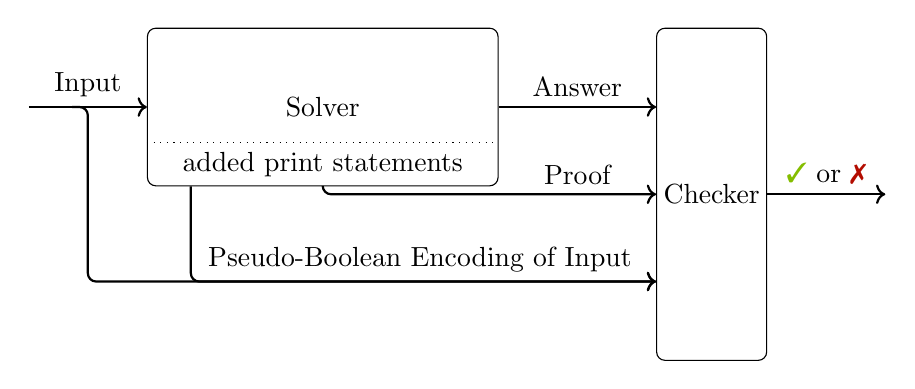
\begin{tikzpicture}
            \node (solver) [inner xsep=5em, inner ysep=2.5em, draw, rounded corners=3pt] { Solver };

            \node (checker) [right=2cm of solver.north east, anchor=north west,
            inner xsep=0.25em, draw, rounded corners=3pt, minimum height=12em, visible on=<3->] { Checker };

            \node (print) [anchor=south, above=0cm of solver.south, visible on=<2->] { added print statements };
            \draw [dotted, visible on=<2->] (solver.west|-print.north) -- (solver.east|-print.north);

            \draw [->, thick] (solver.east) -- (solver.east -| checker.west)
                coordinate [midway] (solutionmid) node [above, midway] { Answer };

            \draw [->, thick, rounded corners=3pt, visible on=<2->] (solver.south) -- (solver.south |- checker.west)
                -- (checker.west) coordinate [midway] (proofmid);

            \coordinate (prooflabel) at (proofmid-|solutionmid);
            \node [above=0cm of prooflabel, visible on=<2->] { Proof };

            \coordinate [right=1.5cm of checker.east] (verified);
            \draw [->, thick, visible on=<5->] (checker.east) -- (verified) node [above, midway] { \textcolor{uofglawn}{\ding{51}} or \textcolor{uofgpillarbox}{\ding{55}} };

            \coordinate [left=1.5cm of solver.west] (input);
            \draw [->, thick] (input) -- (solver.west) coordinate [midway] (inputmid) node [above, midway] { Input };

            \coordinate (checkerbotleft) at ($(checker.west)+($(checker.west)-(solver.east-|checker.west)$)$);

            \draw [->, thick, rounded corners=3pt, visible on=<3>] ($(inputmid)+(-0.2,0)$) --
            (inputmid) -- (inputmid |- checkerbotleft) -- (checkerbotleft) coordinate [midway] (altinputmid);
            \coordinate (solverstart) at ($(solver.south)!0.75!(solver.south west)$);
            \draw [->, thick, rounded corners=3pt, visible on=<4->] (solverstart) -- (solverstart |- checkerbotleft) -- (checkerbotleft);

            \coordinate (encinputlabel) at (altinputmid-|solutionmid);
            \node [above=0cm of encinputlabel, xshift=-2cm, visible on=<4->] { Pseudo-Boolean Encoding of Input };
        \end{tikzpicture}
    \end{center}
\end{frame}

\begin{frame}[fragile,t]{A VeriPB Proof, Attempt One}%
\only<2>{
\begin{tikzpicture}[overlay,remember picture] \coordinate (cliqueheader1space) at ($(pic cs:cliqueheader1)+(0pt,4pt)$); \node[rounded corners, fit = (cliqueheader1space) (pic cs:cliqueheader2) (pic cs:pbcliqueheader1) (pic cs:pbcliqueheader2), fill=uofgsunshine] {};\end{tikzpicture}}%
\only<3>{
\begin{tikzpicture}[overlay,remember picture] \coordinate (opt1space) at ($(pic cs:opt1a)+(0pt,4pt)$); \node[rounded corners, fit = (opt1space) (pic cs:opt1b) (pic cs:pbopt1a) (pic cs:pbopt1b), fill=uofgsunshine] {};\end{tikzpicture}}%
\only<3>{
\begin{tikzpicture}[overlay,remember picture] \coordinate (opt2space) at ($(pic cs:opt2a)+(0pt,4pt)$); \node[rounded corners, fit = (opt2space) (pic cs:opt2b) (pic cs:pbopt2a) (pic cs:pbopt2b), fill=uofgsunshine] {};\end{tikzpicture}}%
\only<4>{
\begin{tikzpicture}[overlay,remember picture] \coordinate (bt1space) at ($(pic cs:bt1a)+(0pt,4pt)$); \node[rounded corners, fit = (bt1space) (pic cs:bt1b) (pic cs:pbbt1a) (pic cs:pbbt1b), fill=uofgsunshine] {};\end{tikzpicture}}%
\only<5>{
\begin{tikzpicture}[overlay,remember picture] \coordinate (bt1space) at ($(pic cs:bt1a)+(0pt,4pt)$); \node[rounded corners, fit = (bt1space) (pic cs:bt1b) (pic cs:pbbt1a) (pic cs:pbbt1b) (pic cs:pbbt3b) (pic cs:pbbt4b), fill=uofgsunshine] {};\end{tikzpicture}}%
\only<5>{
\begin{tikzpicture}[overlay,remember picture] \coordinate (bt5space) at ($(pic
cs:bt5a)+(0pt,4pt)$); \node[rounded corners, fit = (bt5space) (pic cs:bt5b) (pic cs:pbbt5a) (pic
cs:pbbt5b) (pic cs:pbbt6b), fill=uofgsunshine] {};\end{tikzpicture}}%
\only<6>{
\begin{tikzpicture}[overlay,remember picture] \coordinate (bt7space) at ($(pic cs:bt7a)+(0pt,4pt)$); \node[rounded corners, fit = (bt7space) (pic cs:bt7b) (pic cs:pbbt7a) (pic cs:pbbt7b), fill=uofgsunshine] {};\end{tikzpicture}}%
\only<7>{
\begin{tikzpicture}[overlay,remember picture] \coordinate (pbcontpaspace) at ($(pic cs:pbconta)+(0pt,4pt)$); \node[rounded corners, fit = (pic cs:conta) (pbcontpaspace) (pic cs:contb) (pic cs:pbconta) (pic cs:pbcontb), fill=uofgsunshine] {};\end{tikzpicture}}%
\begin{minipage}{0.35\textwidth}
\begin{Verbatim}[commandchars=\\\{\},codes={\catcode`$=3\catcode`^=7}]
\tikzmark{cliqueheader1}maximum clique proof\tikzmark{cliqueheader2}
\tikzmark{opt1a}solution 7 9 12\tikzmark{opt1b}
\tikzmark{bt1a}backtrack 12 7\tikzmark{bt1b}
\tikzmark{bt2a}backtrack 12\tikzmark{bt2b}
\tikzmark{bt3a}backtrack 11 10\tikzmark{bt3b}
\tikzmark{bt4a}backtrack 11\tikzmark{bt4b}
\tikzmark{opt2a}solution 1 2 5 8\tikzmark{opt2b}
\tikzmark{bt5a}backtrack 8 5\tikzmark{bt5b}
\tikzmark{bt6a}backtrack 8\tikzmark{bt6b}
\tikzmark{bt7a}backtrack\tikzmark{bt7b}
\tikzmark{contpa}
\tikzmark{conta}conclusion bounds 4 4
end maximum clique proof\tikzmark{contb}
\end{Verbatim}
\end{minipage}\begin{minipage}{0.45\textwidth}
\begin{Verbatim}[commandchars=\\\{\},codes={\catcode`$=3\catcode`^=7}]
\tikzmark{pbcliqueheader1}pseudo-Boolean proof version 2.0\tikzmark{pbcliqueheader2}
\tikzmark{pbopt1a}@obj soli x7 x9 x12\tikzmark{pbopt1b}
\tikzmark{pbbt1a}rup 1 ~x12 1 ~x7 >= 1 ;\tikzmark{pbbt1b}
rup 1 ~x12 >= 1 ;
rup 1 ~x11 1 ~x10 >= 1 ;\tikzmark{pbbt3b}
rup 1 ~x11 >= 1 ;\tikzmark{pbbt4b}
\tikzmark{pbopt2a}@obj soli x1 x2 x5 x8\tikzmark{pbopt2b}
\tikzmark{pbbt5a}rup 1 ~x8 1 ~x5 >= 1 ;\tikzmark{pbbt5b}
rup 1 ~x8 >= 1 ;\tikzmark{pbbt6b}
\tikzmark{pbbt7a}rup >= 1 ;\tikzmark{pbbt7b}
output NONE\tikzmark{pbconta}
conclusion BOUNDS 8 8
end pseudo-Boolean proof\tikzmark{pbcontb}
\end{Verbatim}
\end{minipage}%
\begin{tikzpicture}[overlay,remember picture]
    \node <1-> [anchor=south east, text depth=2.5cm, rounded corners=3pt, fill=uofgsunshine, draw, yshift=0.9cm, xshift=-0.5cm]
    at (current page.south east) {
        \begin{minipage}[t]{0.3\paperwidth}\raggedright
        \only<1>{Let's try directly translating our ad-hoc proof into VeriPB syntax.}%
        \only<2>{We still start with a header.}%
        \only<3>{The solution command is ``soli''.\\\medskip We put an ``x'' in front of vertex
            numbers, which are now Boolean variables.\\\medskip The
            ``@obj'' is a label, which we'll use later.}%
        \only<4>{To backtrack, we use ``rup''.\\\medskip We're saying ``at least one of these
            variables must be false'', i.e.\ at least one of these vertices must not be selected if we're to
            find a larger clique.}
        \only<5>{Same idea.}
        \only<6>{Backtracking from the root note is saying ``at least one of the variables from
            this empty sum must be true'', i.e.\ asserting contradiction.}
        \only<7>{The ``output'' rule is for advanced features which we're not using, so we have no
            output.
            \\\medskip
            Note we're minimising the number of unselected vertices, so the bound is $12 - 4 =
            8$.}
        \end{minipage}
    };
\end{tikzpicture}
\end{frame}

\begin{frame}[fragile,t]{Verifying This Proof (Or Not\ldots)}
\begin{onlyenv}<1-2>\footnotesize
\begin{Verbatim}
$ veripb example.opb example-1.pbp
Running VeriPB version 2.2.2.post63+git.e70eaf1b
Verification failed.
Failed in proof file line 7.
Hint: Failed to show '1 ~x10 1 ~x11 >= 1' by reverse unit propagation.
\end{Verbatim}
\end{onlyenv}\begin{onlyenv}<3>%
\begin{Verbatim}[commandchars=\\\{\},fontsize=\footnotesize]
$ veripb --trace example.opb example-1.pbp
Running VeriPB version 2.2.2.post63+git.e70eaf1b

=== begin trace ===
  Objective: min 1 ~x12 1 ~x11 1 ~x10 1 ~x9 1 ~x8 1 ~x7 1 ~x6 1 ~x5 1 ~x4 1 ~x3 1 ~x2 1 ~x1 0
  ConstraintId 001 (@noedge1_3): 1 ~x1 1 ~x3 >= 1
  ConstraintId 002 (@noedge2_3): 1 ~x2 1 ~x3 >= 1
...
line 002: @obj soli x12 x7 x9
  ConstraintId 042 (@obj): 1 x1 1 x2 1 x3 1 x4 1 x5 1 x6
                           1 x7 1 x8 1 x9 1 x10 1 x11 1 x12 >= 4
line 003: rup 1 ~x12 1 ~x7 1 ~x9 >= 1 ;
  ConstraintId 043: 1 ~x7 1 ~x9 1 ~x12 >= 1
...
line 006: rup 1 ~x11 1 ~x10 >= 1 ;
Verification failed.
Failed in proof file line 7.
Hint: Failed to show '1 ~x10 1 ~x11 >= 1' by reverse unit propagation.
\end{Verbatim}
\end{onlyenv}\begin{onlyenv}<4>%
\begin{Verbatim}[commandchars=\\\{\},fontsize=\footnotesize]
$ veripb --trace --traceFailed example.opb example-1.pbp
...
line 006: rup 1 ~x11 1 ~x10 >= 1 ;
RUP check failed! The RUP check has the following trace:
  propagations in format '<assignment> (<reason constraint>)':
    ~x12  (1 ~x12 >= 1)
    x11  (1 x10 1 x11 >= 2)
    x10  (1 x10 1 x11 >= 2)
    ~x8  (1 ~x8 1 ~x11 >= 1)
    ~x6  (1 ~x6 1 ~x11 >= 1)
    ~x5  (1 ~x5 1 ~x11 >= 1)
    ~x4  (1 ~x4 1 ~x11 >= 1)
    ~x2  (1 ~x2 1 ~x11 >= 1)
    ~x7  (1 ~x7 1 ~x10 >= 1)

Verification failed.
Failed in proof file line 6.
Hint: Failed to show '1 ~x10 1 ~x11 >= 1' by reverse unit propagation.
\end{Verbatim}
\end{onlyenv}\begin{onlyenv}<5>%
    \begin{itemize}
        \item The proof checker isn't smart enough to figure out that:
            \begin{itemize}
                \item The vertices 1, 3, and 9 can be coloured using one colour\ldots
                \item And each colour class contributes at most one to the objective variable\ldots
                \item So the ``find a clique with more than three vertices'' solution-improving constraint can't be satisfied
                    if we have accepted both 10 and 11.
            \end{itemize}
    \end{itemize}
\end{onlyenv}
\begin{tikzpicture}[overlay,remember picture]
    \node <2-> [anchor=south east, rounded corners=3pt, yshift=0.9cm, xshift=-0.5cm] at (current page.south east) {
        \begin{tikzpicture}
            \begin{scope}[every node/.style = {font=\scriptsize}]
                \myc=1 \advance\myc by -1 \multiply\myc by -360 \divide\myc by 12 \advance\myc by 60
                \node[anchor=center] (L1) at (\the\myc:1.7) {1};
                \node[anchor=center, circle, fill=black, inner sep=2pt] (N1) at (\the\myc:1.42) {};

                \myc=2 \advance\myc by -1 \multiply\myc by -360 \divide\myc by 12 \advance\myc by 60
                \node[anchor=center] (L2) at (\the\myc:1.7) {2};
                \node[anchor=center, circle, fill=black!20, inner sep=2pt] (N2) at (\the\myc:1.42) {};

                \myc=3 \advance\myc by -1 \multiply\myc by -360 \divide\myc by 12 \advance\myc by 60
                \node[anchor=center] (L3) at (\the\myc:1.7) {3};
                \node[anchor=center, circle, fill=black, inner sep=2pt] (N3) at (\the\myc:1.42) {};

                \myc=4 \advance\myc by -1 \multiply\myc by -360 \divide\myc by 12 \advance\myc by 60
                \node[anchor=center] (L4) at (\the\myc:1.7) {4};
                \node[anchor=center, circle, fill=black!20, inner sep=2pt] (N4) at (\the\myc:1.42) {};

                \myc=5 \advance\myc by -1 \multiply\myc by -360 \divide\myc by 12 \advance\myc by 60
                \node[anchor=center] (L5) at (\the\myc:1.7) {5};
                \node[anchor=center, circle, fill=black!20, inner sep=2pt] (N5) at (\the\myc:1.42) {};

                \myc=6 \advance\myc by -1 \multiply\myc by -360 \divide\myc by 12 \advance\myc by 60
                \node[anchor=center] (L6) at (\the\myc:1.7) {6};
                \node[anchor=center, circle, fill=black!20, inner sep=2pt] (N6) at (\the\myc:1.42) {};

                \myc=7 \advance\myc by -1 \multiply\myc by -360 \divide\myc by 12 \advance\myc by 60
                \node[anchor=center] (L7) at (\the\myc:1.7) {7};
                \node[anchor=center, circle, fill=black!20, inner sep=2pt] (N7) at (\the\myc:1.42) {};

                \myc=8 \advance\myc by -1 \multiply\myc by -360 \divide\myc by 12 \advance\myc by 60
                \node[anchor=center] (L8) at (\the\myc:1.7) {8};
                \node[anchor=center, circle, fill=black!20, inner sep=2pt] (N8) at (\the\myc:1.42) {};

                \myc=9 \advance\myc by -1 \multiply\myc by -360 \divide\myc by 12 \advance\myc by 60
                \node[anchor=center] (L9) at (\the\myc:1.7) {9};
                \node[anchor=center, circle, fill=black, inner sep=2pt] (N9) at (\the\myc:1.42) {};

                \myc=10 \advance\myc by -1 \multiply\myc by -360 \divide\myc by 12 \advance\myc by 60
                \node[anchor=center] (L10) at (\the\myc:1.7) {10};
                \node[anchor=center, circle, fill=uofgthistle, inner sep=2pt] (N10) at (\the\myc:1.42) {};

                \myc=11 \advance\myc by -1 \multiply\myc by -360 \divide\myc by 12 \advance\myc by 60
                \node[anchor=center] (L11) at (\the\myc:1.7) {11};
                \node[anchor=center, circle, fill=uofgthistle, inner sep=2pt] (N11) at (\the\myc:1.42) {};

                \myc=12 \advance\myc by -1 \multiply\myc by -360 \divide\myc by 12 \advance\myc by 60
                \node[anchor=center] (L12) at (\the\myc:1.7) {\phantom{12}};

                \draw [color=black!20] (N1) -- (N2);
                \draw [color=black!20] (N1) -- (N5);
                \draw [color=black!20] (N1) -- (N8);
                \draw (N1) -- (N10);
                \draw (N1) -- (N11);
                \draw [color=black!20] (N2) -- (N5);
                \draw [color=black!20] (N2) -- (N8);
                \draw [color=black!20] (N2) -- (N10);
                \draw [color=black!20] (N3) -- (N4);
                \draw [color=black!20] (N3) -- (N6);
                \draw (N3) -- (N10);
                \draw (N3) -- (N11);
                \draw [color=black!20] (N4) -- (N6);
                \draw [color=black!20] (N5) -- (N8);
                \draw [color=black!20] (N6) -- (N7);
                \draw [color=black!20] (N7) -- (N9);
                \draw [color=black!20] (N7) -- (N11);
                \draw [color=black!20] (N8) -- (N9);
                \draw (N9) -- (N10);
                \draw (N9) -- (N11);
                \draw [ultra thick, color=uofgthistle] (N10) -- (N11);
            \end{scope}
        \end{tikzpicture}
    };
\end{tikzpicture}
\end{frame}

\begin{frame}[fragile,t]{Colour Classes are At-Most-One Constraints}%
\begin{onlyenv}<1-4>%
        If we could take the ``objective improving'' constraint
\begin{Verbatim}[commandchars=\\\{\},fontsize=\scriptsize]
line 003: @obj soli x12 x7 x9
  ConstraintId 042 (@obj): 1 x1 1 x2 1 x3 1 x4 1 x5 1 x6 1 x7 1 x8 1 x9 1 x10 1 x11 1 x12 >= 4
\end{Verbatim}
            i.e. \[
                x_1 + x_2 + x_3 + x_4 + x_5 + x_6 + x_7 + x_8 + x_9 + x_{10} + x_{11} + x_{12} \ge 4
            \]
            \pause
            and add an at-most-one constraint over the colour class $\{x_1, x_3, x_9\}$,
            \[\overline{x}_1 + \overline{x}_3 + \overline{x}_9 \ge 2\]
            \pause
we would get \[
    (x_1 + \overline{x}_1) + x_2 + (x_3 + \overline{x}_3) + x_4 + x_5 + x_6 + x_7 + x_8 + (x_9 +
            \overline{x}_9) + x_{10} + x_{11} + x_{12} \ge 6\]
        \pause
        and simplifying using $x_i + \overline{x}_i = 1$ we get \[
    x_2 + x_4 + x_5 + x_6 + x_7 + x_8 + x_{10} + x_{11} + x_{12} \ge 3\]
from which it is much easier to see that taking both vertices 10 and 11 isn't going to work.
\end{onlyenv}\begin{onlyenv}<5>%

\begin{tikzpicture}[overlay,remember picture] \coordinate (assert1aspace) at ($(pic cs:assert1a)+(0pt,4pt)$); \node[rounded corners, fit = (assert1aspace) (pic cs:assert1b), fill=uofgsunshine] {};\end{tikzpicture}%

\begin{tikzpicture}[overlay,remember picture] \coordinate (assert2aspace) at ($(pic cs:assert2a)+(0pt,4pt)$); \node[rounded corners, fit = (assert2aspace) (pic cs:assert2b), fill=uofglawn] {};\end{tikzpicture}%
\begin{Verbatim}[commandchars=\\\{\},codes={\catcode`$=3\catcode`^=7}]
pseudo-Boolean proof version 2.0
@obj soli x7 x9 x12
rup 1 ~x12 1 ~x7 >= 1 ;
rup 1 ~x12 >= 1 ;
\tikzmark{assert1a}a 1 x2 1 x4 1 x5 1 x6 1 x7 1 x8 1 x10 1 x11 1 x12 >= 3 ;\tikzmark{assert1b}
rup 1 ~x11 1 ~x10 >= 1 ;
rup 1 ~x11 >= 1 ;
@obj soli x1 x2 x5 x8
rup 1 ~x8 1 ~x5 >= 1 ;
rup 1 ~x8 >= 1 ;
\tikzmark{assert2a}a 1 x8 1 x11 1 x12 >= 2 ;\tikzmark{assert2b}
rup >= 1 ;
output NONE
conclusion BOUNDS 8 8
end pseudo-Boolean proof
\end{Verbatim}
\begin{tikzpicture}[overlay,remember picture]
    \node [anchor=north east, text depth=0.6cm, rounded corners=3pt, fill=uofgsunshine, draw, yshift=-2.5cm, xshift=-0.5cm]
    at (current page.north east) {
        \begin{minipage}[t]{0.5\paperwidth}\raggedright
            The ``a'' means ``I'm asserting this without a justification.''
        \end{minipage}
    };
\end{tikzpicture}%
\begin{tikzpicture}[overlay,remember picture]
    \node [anchor=south east, text depth=1.4cm, rounded corners=3pt, fill=uofglawn, draw, yshift=0.9cm, xshift=-0.5cm]
    at (current page.south east) {
        \begin{minipage}[t]{0.5\paperwidth}\raggedright
            It turns out we'll need to help here too. This time we're dealing with three colour
            classes, each of three vertices. Note that this isn't obvious from the constraint
            we're asserting\ldots
        \end{minipage}
    };
\end{tikzpicture}%
\end{onlyenv}\begin{onlyenv}<6>%
\begin{Verbatim}
$ veripb example.opb example-2.pbp
Running VeriPB version 2.2.2.post63+git.e70eaf1b
s VERIFIED BOUNDS 8 <= obj <= 8
WARNING:root:Proof is based on unjustified assumptions.
Verification succeeded.
\end{Verbatim}

\bigskip

This passes, but the checker complains about our use of the ``a'' rule.

\bigskip

This is fair: it's really not obvious that the constraints we specify are valid. In general, we
might have worked very hard to produce a good colour bound.
\end{onlyenv}\begin{onlyenv}<7>%
\vspace*{-0.6cm}%

\begin{tikzpicture}[overlay,remember picture] \coordinate (assert3aspace) at ($(pic cs:assert3a)+(0pt,4pt)$); \node[rounded corners, fit = (assert3aspace) (pic cs:assert3b) (pic cs:assert3c), fill=uofgsunshine] {};\end{tikzpicture}%

\begin{tikzpicture}[overlay,remember picture] \coordinate (assert4aspace) at ($(pic cs:assert4a)+(0pt,4pt)$); \node[rounded corners, fit = (assert4aspace) (pic cs:assert4b) (pic cs:assert4c) (pic cs:assert4d), fill=uofglawn] {};\end{tikzpicture}%
\begin{Verbatim}[commandchars=\\\{\},codes={\catcode`$=3\catcode`^=7},fontsize=\footnotesize]
pseudo-Boolean proof version 2.0
@obj soli x7 x9 x12
rup 1 ~x12 1 ~x7 >= 1 ;
rup 1 ~x12 >= 1 ;
\tikzmark{assert3a}a 1 ~x1 1 ~x3 1 ~x9 >= 2 ;\tikzmark{assert3b}
pol @obj -1 +\tikzmark{assert3c}
rup 1 ~x11 1 ~x10 >= 1 ;
rup 1 ~x11 >= 1 ;
@obj soli x1 x2 x5 x8
rup 1 ~x8 1 ~x5 >= 1 ;
rup 1 ~x8 >= 1 ;
\tikzmark{assert4a}a 1 ~x1 1 ~x3 1 ~x7 >= 2 ;\tikzmark{assert4b}
a 1 ~x2 1 ~x4 1 ~x9 >= 2 ;
a 1 ~x5 1 ~x6 1 ~x10 >= 2 ;\tikzmark{assert4c}
pol @obj -1 + -2 + -3 +\tikzmark{assert4d}
rup >= 1 ;
output NONE
conclusion BOUNDS 8 8
end pseudo-Boolean proof
\end{Verbatim}
\begin{tikzpicture}[overlay,remember picture]
    \node [anchor=north east, text depth=1.4cm, rounded corners=3pt, fill=uofgsunshine, draw, yshift=-2.5cm, xshift=-0.5cm]
    at (current page.north east) {
        \begin{minipage}[t]{0.5\paperwidth}\raggedright
            ``pol'' means ``reverse Polish notation''. So, take the solution-improving constraint we
            labelled ``@obj'', and add the previous constraint (negative numbers are relative to the
            current constraint).
        \end{minipage}
    };
\end{tikzpicture}%
\begin{tikzpicture}[overlay,remember picture]
    \node [anchor=south east, text depth=1.0cm, rounded corners=3pt, fill=uofglawn, draw, yshift=0.9cm, xshift=-0.5cm]
    at (current page.south east) {
        \begin{minipage}[t]{0.5\paperwidth}\raggedright
            Here we're asserting at-most-one constraints for three colour classes, and then adding
            all of them to the solution-improving constraint.
        \end{minipage}
    };
\end{tikzpicture}%
\end{onlyenv}\begin{onlyenv}<8>%
\begin{Verbatim}
$ veripb example.opb example-3.pbp
Running VeriPB version 2.2.2.post63+git.e70eaf1b
s VERIFIED BOUNDS 8 <= obj <= 8
WARNING:root:Proof is based on unjustified assumptions.
Verification succeeded.
\end{Verbatim}

\bigskip

Still relying upon assertions, but ``these vertices form a colour class'' is easily verifiable.
\end{onlyenv}
\end{frame}

\begin{frame}{Why a General-Purpose Proof System?}
    Why not have a ``colouring bound'' rule directly in the proof format?
    \begin{itemize}
        \item Dozens of different colouring algorithms, and extensions using MaxSAT-like reasoning.
        \item Even more when we look at problems like maximum weight clique.
            Weighted colour class rules can be extremely clever (e.g. vertices can split their weights
            between multiple colours).
        \item Don't really want to have a proof checker per solver if we can help it\ldots
    \end{itemize}
    Fortunately, this isn't necessary.
\end{frame}

\begin{frame}[fragile]{Recovering At-Most-One Constraints}
\begin{onlyenv}<1-6>
    We can lazily recover at-most-one constraints for each colour class!
    \uncover<2->{
      \begin{align*}
        (\overline{x}_1 + \overline{x}_6 \ge 1) & \\
        +\,(\overline{x}_1 + \overline{x}_9 \ge 1) & &=~&
2 \overline{x}_1 +
\hphantom{2} \overline{x}_6 +
\hphantom{2} \overline{x}_9
\ge 2~ \\
        +\,(\overline{x}_6 + \overline{x}_9 \ge 1) & &=~&
2 \overline{x}_1 +
2 \overline{x}_6 +
2 \overline{x}_9
  \ge 3 \\\uncover<3->{
        /\,2
& &=~&
\hphantom{2} \overline{x}_1 +
\hphantom{2} \overline{x}_6 +
\hphantom{2} \overline{x}_9
          \ge\uncover<3->{\only<1-3>{{\frac{3}{2}}}\only<4->{2\vphantom{\frac{3}{2}}}} \\
          && \uncover<5->{\text{i.e.}~ & x_1 + x_6 + x_9 \le 1}}
    \end{align*}}
  \uncover<6->{
    This generalises
    to colour classes of any size~$v$.
    \begin{itemize}
        \item
          Each non-edge is used exactly once, $v (v - 1)$ additions
        \item
          $v - 3$ multiplications and $v-2$ divisions.
    \end{itemize}
    Solvers don't need to ``understand'' why this works (or when exactly it is necessary) to
    write this derivation to proof log.
}
\end{onlyenv}\begin{onlyenv}<7>

\begin{tikzpicture}[overlay,remember picture] \coordinate (recover1aspace) at ($(pic cs:recover1a)+(0pt,4pt)$); \node[rounded corners, fit = (recover1aspace) (pic cs:recover1b), fill=uofgsunshine] {};\end{tikzpicture}%

\begin{tikzpicture}[overlay,remember picture] \coordinate (recover2aspace) at ($(pic cs:recover2a)+(0pt,4pt)$); \node[rounded corners, fit = (recover2aspace) (pic cs:recover2b), fill=uofgsunshine] {};\end{tikzpicture}%

\begin{tikzpicture}[overlay,remember picture] \coordinate (recover3aspace) at ($(pic cs:recover3a)+(0pt,4pt)$); \node[rounded corners, fit = (recover3aspace) (pic cs:recover3b), fill=uofgsunshine] {};\end{tikzpicture}%

\begin{tikzpicture}[overlay,remember picture] \coordinate (recover4aspace) at ($(pic cs:recover4a)+(0pt,4pt)$); \node[rounded corners, fit = (recover4aspace) (pic cs:recover4b) (pic cs:recover4c), fill=uofglawn] {};\end{tikzpicture}%
\vspace*{-0.6cm}
\begin{Verbatim}[commandchars=\\\{\},codes={\catcode`$=3\catcode`^=7},fontsize=\footnotesize]
pseudo-Boolean proof version 2.0
@obj soli x12 x7 x9
rup 1 ~x12 1 ~x7 1 ~x9 >= 1 ;
rup 1 ~x12 1 ~x7 >= 1 ;
\tikzmark{recover1a}pol @noedge1_6 @noedge1_9 + @noedge6_9 + 2 d @obj +\tikzmark{recover1b}
rup 1 ~x12 >= 1 ;
\tikzmark{recover2a}pol @noedge1_3 @noedge1_9 + @noedge3_9 + 2 d @obj +\tikzmark{recover2b}
rup 1 ~x11 1 ~x10 >= 1 ;
\tikzmark{recover3a}pol @noedge1_3 @noedge1_7 + @noedge3_7 + 2 d @obj +\tikzmark{recover3b}
rup 1 ~x11 >= 1 ;
@obj soli x8 x5 x2 x1
rup 1 ~x8 1 ~x5 >= 1 ;
pol @obj @noedge1_9 +
rup 1 ~x8 >= 1 ;
\tikzmark{recover4a}pol @noedge1_3 @noedge1_7 + @noedge3_7 + 2 d @noedge2_4 @noedge2_9 + @noedge4_9 + 2 d +\tikzmark{recover4b}
    @noedge5_6 @noedge5_10 + @noedge6_10 + 2 d + @obj +\tikzmark{recover4c}
rup >= 1 ;
output NONE
conclusion BOUNDS 8 8
end pseudo-Boolean proof
\end{Verbatim}
\begin{tikzpicture}[overlay,remember picture]
    \node [anchor=north east, text depth=3.2cm, rounded corners=3pt, fill=uofgsunshine, draw, yshift=-1.5cm, xshift=-0.5cm]
    at (current page.north east) {
        \begin{minipage}[t]{0.4\paperwidth}\raggedright
            It turns out we do colour-class reasoning in each of these three places, although the
            verifier actually doesn't need help with the first two.\\ \medskip
            In each case, we add together three non-adjacency constraints, divide by two, and then
            add the result to the solution-\\improving constraint.
        \end{minipage}
    };
\end{tikzpicture}%
\begin{tikzpicture}[overlay,remember picture]
    \node [anchor=south east, text depth=0.5cm, rounded corners=3pt, fill=uofglawn, draw, yshift=0.6cm, xshift=-0.5cm]
    at (current page.south east) {
        \begin{minipage}[t]{0.6\paperwidth}\raggedright
            Here we're creating three at-most-one constraints, and then
            adding all of them to the solution-improving constraint.
        \end{minipage}
    };
\end{tikzpicture}%
\end{onlyenv}\begin{onlyenv}<8>
\begin{Verbatim}
$ veripb example.opb example.pbp
Running VeriPB version 2.2.2.post63+git.e70eaf1b
s VERIFIED BOUNDS 8 <= obj <= 8
Verification succeeded.
\end{Verbatim}
\end{onlyenv}
\end{frame}

\section{VeriPB Proofs}

\begin{frame}{What is RUP, Anyway?}
\end{frame}

\begin{frame}{Cutting Planes}
\end{frame}

\begin{frame}{Not Appearing in this Talk}
    \begin{itemize}
        \item Extension variables (and dominance and symmetries).
        \item Deletions.
    \end{itemize}
\end{frame}

\section{End-to-End Verification}

\subsection{Gocht, McCreesh, Myreen, Nordstr\"om, Oertel, Tan: End-to-End Verification for Subgraph Solving, AAAI 2024}

\begin{frame}{Reducing the Trust Base}
    \begin{center}
        \begin{tikzpicture}
            \node (solver) [ inner xsep=4em, inner ysep=2.5em, draw, rounded corners=3pt] { Solver };
            \node (elaborator) [ right=2cm of solver.north east, anchor=north west, inner
            xsep=0.25em, draw, rounded corners=3pt, minimum height=12em, text width=5em, text centered] {
                \only<1>{Checker}\only<2->{Elaborator} };
            \node (verifiedchecker) [ right=2cm of elaborator.north east, anchor=north west, inner
                xsep=0.25em, draw, rounded corners=3pt, minimum height=8em, text width=4em, text
                centered, yshift=-2cm, visible on=<3->] { Verified Checker };

            \node (print) [anchor=south, above=0cm of solver.south] { added print statements };
            \draw [dotted] (solver.west|-print.north) -- (solver.east|-print.north);

            \draw [->, thick] (solver.east) -- (solver.east -| elaborator.west) coordinate [midway]
            (solutionmid) node [above, midway] { Answer };

            \draw [->, thick, rounded corners=3pt] (solver.south) -- (solver.south |- elaborator.west) -- (elaborator.west) coordinate [midway] (proofmid);

            \coordinate (prooflabel) at (proofmid-|solutionmid); \node [above=0cm of prooflabel] { Proof };

            \coordinate [right=2cm of verifiedchecker.east] (verified);
            \draw [->, thick, visible on=<3>] (verifiedchecker.east) -- (verified)
                node [above, midway] { \textcolor{uofglawn}{\ding{51}} or \textcolor{uofgpillarbox}{\ding{55}} }
                node [below, midway, text centered, text width=5em] { Trusted Answer };
            \draw [->, thick, visible on=<4>] (verifiedchecker.east) -- (verified)
                node [above, midway] { \textcolor{uofglawn}{\ding{51}} or \textcolor{uofgpillarbox}{\ding{55}} }
                node [below, midway, text centered, text width=5em] { Trusted Answer in Graph Language };

            \coordinate [left=1.5cm of solver.west] (input);
            \draw [->, thick] (input) -- (solver.west) coordinate [midway] (inputmid) node [above, midway] { Input };

            \coordinate (verifiedcheckertopleft) at ($(verifiedchecker.west)+($(0cm,1.2cm)$)$);
            \draw [->, thick, visible on=<2->] (elaborator.east |- verifiedcheckertopleft) --
            (verifiedcheckertopleft) node [above, midway, text width=4em, text centered] { Answer };
            \draw [->, thick, visible on=<2->] (elaborator.east |- verifiedchecker.west) -- (verifiedchecker.west) node [above, midway, text width=4em, text centered] { Kernel Proof };

            \coordinate (elaboratorbotleft) at ($(elaborator.west)+($(elaborator.west)-(solver.east-|elaborator.west)$)$);
            \coordinate (verifiedcheckerbotleft) at ($(verifiedchecker.west)+($(0cm,-1.2cm)$)$);

            \coordinate (elaboratortopright) at ($(elaborator.east)+($(verifiedcheckertopleft)-(verifiedchecker.west)$)$);
            \draw [->, thick] (elaboratortopright) -- (elaboratortopright-|verifiedchecker.west)
                node [above, midway] { \textcolor{uofglawn}{\ding{51}} or \textcolor{uofgpillarbox}{\ding{55}} };

            \coordinate (solverstart) at ($(solver.south)!0.75!(solver.south west)$);
            \coordinate (checkerbotleft) at ($(elaborator.west)+($(elaborator.west)-(solver.east-|elaborator.west)$)$);
            \draw [->, thick, rounded corners=3pt] (solverstart) -- (solverstart |- checkerbotleft) -- (checkerbotleft)
            coordinate [midway] (altinputmid);

            \coordinate (encinputlabel) at (altinputmid-|solutionmid);
            \node [above=0cm of encinputlabel, xshift=-0.5cm] { Encoded Input };

            \draw [->, thick, rounded corners=3pt, visible on=<3>] (solverstart) -- (solverstart |- verifiedcheckerbotleft) -- (verifiedcheckerbotleft);
            \draw [->, thick, rounded corners=3pt, visible on=<4>] ($(inputmid)+(-0.2,0)$) --
            (inputmid) -- (inputmid |- verifiedcheckerbotleft) -- (verifiedcheckerbotleft)
            coordinate [midway] (verinputmid);

            \coordinate (verinputlabel) at (verinputmid-|solutionmid);
            \node [above=0cm of verinputlabel, xshift=-0.5cm, visible on=<4>] { Verified Input };
        \end{tikzpicture}
    \end{center}
\end{frame}

\begin{frame}[fragile]{End-to-End Verification for Maximum Clique}\vspace*{-0.3cm}
\begin{Verbatim}[fontsize=\footnotesize]
$ glasgow_clique_solver brock200_4.clq
recursions = 56613
omega = 17
clique = 12 19 28 29 38 54 65 71 79 93 117 127 139 161 165 186 192
runtime = 0.02153s

$ glasgow_clique_solver brock200_4.clq --prove brock200_4
runtime = 0.266475s

$ veripb --stats brock200_4.opb brock200_4.pbp
s VERIFIED BOUNDS 183 <= obj <= 183
c statistic: time total: 15.31s

$ cake_pb_clique brock200_4.clq > brock200_4.verifiedopb

$ veripb --stats brock200_4.verifiedopb brock200_4.pbp --proofOutput brock200_4.corepb
s VERIFIED BOUNDS 183 <= obj <= 183
c statistic: time total: 17.28s

$ time cake_pb_clique brock200_4.clq brock200_4.corepb
s VERIFIED MAX CLIQUE SIZE |CLIQUE| = 17
real    0m2.260s
\end{Verbatim}
\end{frame}

\begin{frame}{What Exactly are we Verifying?}
    \only<1>{
    \begin{holthmenv}
    \HOLConst{is_clique}\;\HOLFreeVar{vs}\;(\HOLFreeVar{v}\HOLSymConst{,}\HOLFreeVar{e})\;\HOLTokenDefEquality{}\\
    \;\;\HOLFreeVar{vs}\;\HOLSymConst{\HOLTokenSubset{}}\;\HOLcount{\HOLFreeVar{v}}\;\HOLSymConst{\HOLTokenConj{}}\\
    \;\;\HOLSymConst{\HOLTokenForall{}}\HOLBoundVar{x}\;\HOLBoundVar{y}.\;\HOLBoundVar{x}\;\HOLSymConst{\HOLTokenIn{}}\;\HOLFreeVar{vs}\;\HOLSymConst{\HOLTokenConj{}}\;\HOLBoundVar{y}\;\HOLSymConst{\HOLTokenIn{}}\;\HOLFreeVar{vs}\;\HOLSymConst{\HOLTokenConj{}}\;\HOLBoundVar{x}\;\HOLSymConst{\HOLTokenNotEqual{}}\;\HOLBoundVar{y}\;\HOLSymConst{\HOLTokenImp{}}\;\HOLConst{is_edge}\;\HOLFreeVar{e}\;\HOLBoundVar{x}\;\HOLBoundVar{y}
    \end{holthmenv}

    \begin{holthmenv}
    \HOLConst{max_clique_size}\;\HOLFreeVar{g}\;\HOLTokenDefEquality{}\;\HOLConst{max\ensuremath{_{\text{set}}}}\;\HOLTokenLeftbrace{}\HOLConst{card}\;\HOLBoundVar{vs}\;\HOLTokenBar{}\;\HOLConst{is_clique}\;\HOLBoundVar{vs}\;\HOLFreeVar{g}\HOLTokenRightbrace{}
    \end{holthmenv}
}\only<2>{
\begin{holthmenv}
\HOLConst{clique_eq_str}\;\HOLFreeVar{n}\;\HOLTokenDefEquality{}\;\HOLStringLitDG{s VERIFIED MAX CLIQUE SIZE |CLIQUE| = }\;\HOLSymConst{\^{}}\;\HOLConst{toString}\;\HOLFreeVar{n}\;\HOLSymConst{\^{}}\;\HOLStringLitDG{\HOLTokenBackslash{}n}
\end{holthmenv}

\begin{holthmenv}
\HOLConst{clique_bound_str}\;\HOLFreeVar{l}\;\HOLFreeVar{u}\;\HOLTokenDefEquality{}\\
\;\;\HOLStringLitDG{s VERIFIED MAX CLIQUE SIZE BOUND }\;\HOLSymConst{\^{}}\;\HOLConst{toString}\;\HOLFreeVar{l}\;\HOLSymConst{\^{}}\;\HOLStringLitDG{ <= |CLIQUE| <= }\;\HOLSymConst{\^{}}\;\HOLConst{toString}\;\HOLFreeVar{u}\;\HOLSymConst{\^{}}\;\HOLStringLitDG{\HOLTokenBackslash{}n}
\end{holthmenv}

\begin{holthmenv}
\HOLTokenTurnstile{}\;\HOLConst{cake_pb_clique_run}\;\HOLFreeVar{cl}\;\HOLFreeVar{fs}\;\HOLFreeVar{mc}\;\HOLFreeVar{ms}\;\HOLSymConst{\HOLTokenImp{}}\\
\;\;\;\;\;\HOLConst{machine_sem}\;\HOLFreeVar{mc}\;(\HOLConst{basis_ffi}\;\HOLFreeVar{cl}\;\HOLFreeVar{fs})\;\HOLFreeVar{ms}\;\HOLSymConst{\HOLTokenSubset{}}\\
\;\;\;\;\;\;\;\HOLConst{extend_with_resource_limit}\;\HOLTokenLeftbrace{}\HOLConst{Terminate}\;\HOLConst{Success}\;(\HOLConst{cake_pb_clique_io_events}\;\HOLFreeVar{cl}\;\HOLFreeVar{fs})\HOLTokenRightbrace{}\;\HOLSymConst{\HOLTokenConj{}}\\
\;\;\;\;\;\HOLSymConst{\HOLTokenExists{}}\HOLBoundVar{out}\;\HOLBoundVar{err}.\\
\;\;\;\;\;\;\;\HOLConst{extract_fs}\;\HOLFreeVar{fs}\;(\HOLConst{cake_pb_clique_io_events}\;\HOLFreeVar{cl}\;\HOLFreeVar{fs})\;\HOLSymConst{=}\;\HOLConst{Some}\;(\HOLConst{add_stdout}\;(\HOLConst{add_stderr}\;\HOLFreeVar{fs}\;\HOLBoundVar{err})\;\HOLBoundVar{out})\;\HOLSymConst{\HOLTokenConj{}}\\
\;\;\;\;\;\;\;(\HOLBoundVar{out}\;\HOLSymConst{\HOLTokenNotEqual{}}\;\HOLStringLitDG{}\;\HOLSymConst{\HOLTokenImp{}}\\
\;\;\;\;\;\;\;\;\;\;\HOLSymConst{\HOLTokenExists{}}\HOLBoundVar{g}.\;\HOLConst{get_graph_dimacs}\;\HOLFreeVar{fs}\;(\HOLConst{el}\;\HOLNumLit{1}\;\HOLFreeVar{cl})\;\HOLSymConst{=}\;\HOLConst{Some}\;\HOLBoundVar{g}\;\HOLSymConst{\HOLTokenConj{}}\\
\;\;\;\;\;\;\;\;\;\;\;\;\;\;(\HOLConst{length}\;\HOLFreeVar{cl}\;\HOLSymConst{=}\;\HOLNumLit{2}\;\HOLSymConst{\HOLTokenConj{}}\;\HOLBoundVar{out}\;\HOLSymConst{=}\;\HOLConst{concat}\;(\HOLConst{print_pbf}\;(\HOLConst{full_encode}\;\HOLBoundVar{g}))\;\HOLSymConst{\HOLTokenDisj{}}\\
\;\;\;\;\;\;\;\;\;\;\;\;\;\;\;\HOLConst{length}\;\HOLFreeVar{cl}\;\HOLSymConst{=}\;\HOLNumLit{3}\;\HOLSymConst{\HOLTokenConj{}}\\
\;\;\;\;\;\;\;\;\;\;\;\;\;\;\;\;\;\;\;(\HOLBoundVar{out}\;\HOLSymConst{=}\;\HOLConst{clique_eq_str}\;(\HOLConst{max_clique_size}\;\HOLBoundVar{g})\;\HOLSymConst{\HOLTokenDisj{}}\\
\;\;\;\;\;\;\;\;\;\;\;\;\;\;\;\;\;\;\;\HOLSymConst{\HOLTokenExists{}}\HOLBoundVar{l}\;\HOLBoundVar{u}.\HOLBoundVar{out}\;\HOLSymConst{=}\;\HOLConst{clique_bound_str}\;\HOLBoundVar{l}\;\HOLBoundVar{u}\;\HOLSymConst{\HOLTokenConj{}}\;(\HOLSymConst{\HOLTokenForall{}}\HOLBoundVar{vs}.\;\HOLConst{is_clique}\;\HOLBoundVar{vs}\;\HOLBoundVar{g}\;\HOLSymConst{\HOLTokenImp{}}\;\HOLConst{card}\;\HOLBoundVar{vs}\;\HOLSymConst{\HOLTokenLeq{}}\;\HOLBoundVar{u})\;\HOLSymConst{\HOLTokenConj{}}\\
\;\;\;\;\;\;\;\;\;\;\;\;\;\;\;\;\;\;\;\;\;\;\;\;\;\;\HOLSymConst{\HOLTokenExists{}}\HOLBoundVar{vs}.\;\HOLConst{is_clique}\;\HOLBoundVar{vs}\;\HOLBoundVar{g}\;\HOLSymConst{\HOLTokenConj{}}\;\HOLBoundVar{l}\;\HOLSymConst{\HOLTokenLeq{}}\;\HOLConst{card}\;\HOLBoundVar{vs})))
\end{holthmenv}}
\end{frame}

\begin{frame}{What's Left to Trust?}
    Still have to trust:
    \begin{itemize}
        \item The HOL4 theorem prover.
        \item That the formal HOL model of the CakeML environment corresponds to the
            hardware on which it is run.
        \item HOL definition of what it means to be a maximum clique.
        \item Input parsing and output formatting.
    \end{itemize}

    \bigskip

    No need to trust, or even know about:
    \begin{itemize}
        \item How the solver works.
        \item What pseudo-Boolean means.
    \end{itemize}
\end{frame}

\begin{frame}{Code}
  \begin{center}
    \url{https://github.com/ciaranm/glasgow-subgraph-solver}

      \bigskip

    \url{https://gitlab.com/MIAOresearch/software/VeriPB}

      \bigskip

      \url{https://gitlab.com/MIAOresearch/software/CakePB}
  \end{center}
\end{frame}

\section{Subgraph Isomorphism}

\section{Tricker Things}

\section{Conclusion}

\begin{frame}{Conclusion}
    \begin{itemize}
        \item Need to be able to express a wide range of reasoning rules, efficiently.
        \item Cutting planes can do this (which is somewhat mysterious).
        \item Mixing RUP and explicit inference rules makes proofs much easier to write.
    \end{itemize}
\end{frame}

{
    \usebackgroundtemplate{
        \tikz[overlay, remember picture]
        \node[at=(current page.south), anchor=south, yshift=-1cm, inner sep=0pt]{\includegraphics[keepaspectratio=true, width=\paperwidth]{../../images/background2.jpg}};
    }

    \begin{frame}[plain,noframenumbering]
        \begin{tikzpicture}[remember picture, overlay]
            \node at (current page.north west) {
                \begin{tikzpicture}[remember picture, overlay]
                    \fill [fill=uofguniversityblue, anchor=north west] (0, 0) rectangle (\paperwidth, -2.8cm);
                \end{tikzpicture}
            };

            \node (logo) [anchor=north east, shift={(-0.8cm,-0.2cm)}] at (current page.north east) {
                
\includegraphics[keepaspectratio=true,scale=0.5]{../../images/UoG_keyline.pdf}
            };

            \node (logo2) [anchor=north, below=0.2cm of logo.south] {
                
\includegraphics[keepaspectratio=true,scale=0.1]{../../images/RAEngWhite.pdf}
            };

            \coordinate (logos) at ($(logo.south)!0.5!(logo2.north)$);

            \node [anchor=west, xshift=0.8cm] at (current page.west |- logos) {
                \begin{minipage}{0.60\paperwidth}\raggedright
                    \textcolor{white}{\url{https://ciaranm.github.io/}} \\[0.3cm]
                    \textcolor{white}{\href{mailto:ciaran.mccreesh@glasgow.ac.uk}{\nolinkurl{ciaran.mccreesh@glasgow.ac.uk}}}
                \end{minipage}
            };
        \end{tikzpicture}
    \end{frame}
}

\end{document}

